\chapter{实验设计与结果分析}

\section{实验环境与评价方法}

\subsection{实验环境配置}

实验在 Ubuntu 22.04 LTS 操作系统上进行，硬件配备 x86\_64 架构 CPU 和一块 24 GB 显存的 NVIDIA RTX 4090 GPU。软件方面，通过 Conda 构建独立的 Python 3.10 虚拟环境，并安装与 CUDA 版本兼容的 PyTorch 作为核心深度学习框架。该环境既能满足原始 FennOmix.MHC 模型的复现要求，也为后续的降维、剪枝、缓存压缩及索引实现提供了统一的实验基础。

所有模型的训练与测试均在同一环境下完成。训练采用 SiameseCELoss 作为损失函数，优化器选用 Adam，基础学习率设置为： $ \eta = 1 \times 10^{-4}$ 。

实验不另外从训练集切分验证集，而是直接使用独立测试集进行周期性评估，并将训练损失、测试召回率等指标记录至 SwanLab，以便对比不同模型配置下的性能变化。

\begin{figure}[htbp]
    \centering
    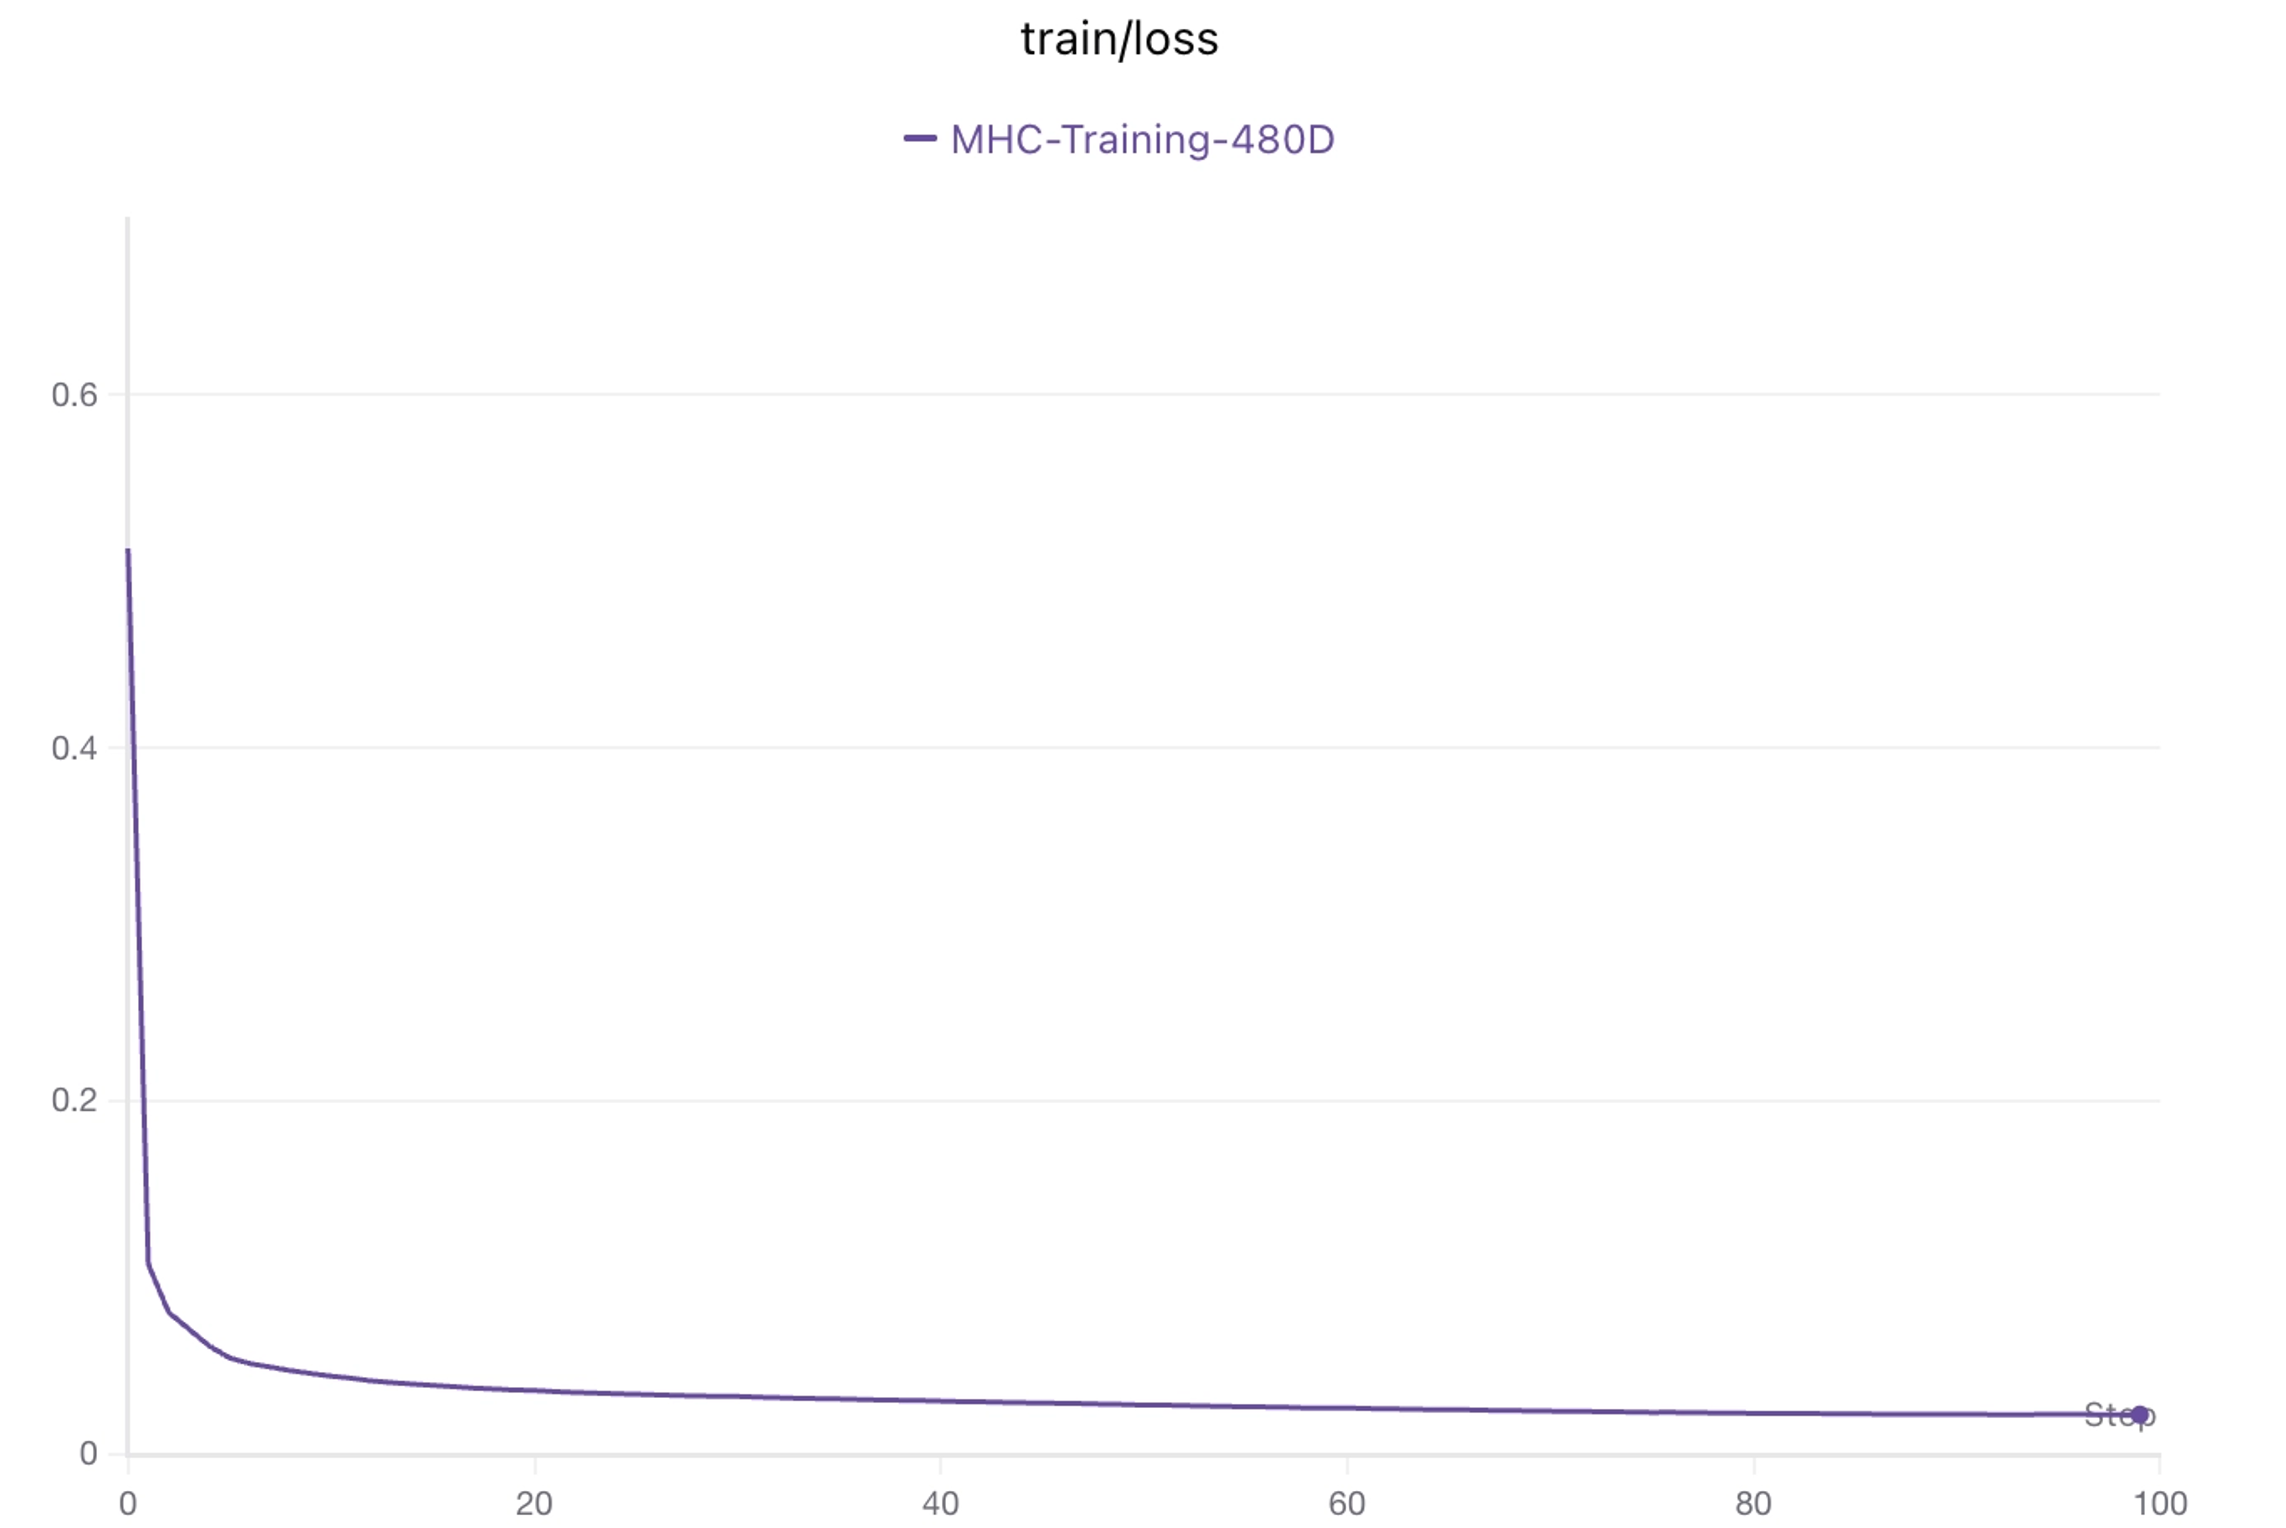
\includegraphics[width=0.70\textwidth]{figures/training_curve.png}
    \caption{训练过程曲线}
    \label{fig:training-curve}
\end{figure}

图~\ref{fig:training-curve} 绘制了训练过程中的主要指标曲线。整体趋势显示模型训练过程平稳，测试指标未见显著异常波动，表明实验环境与复现流程能够支撑后续的模型优化实验。

\subsection{任务设置}

实验围绕 FennOmix.MHC 的复现与部署优化展开，涵盖四类主要任务：其一，复现原始模型的训练和测试流程；其二，考察不同输出维度对模型性能及缓存成本的影响；其三，比较 Linear 与 MLP 两种 64 维降维模型在常规指标和下游缩库辅助搜库任务中的表现；其四，检验剪枝、INT8 量化压缩以及索引加载机制对系统部署的作用。

在大规模部署背景下，考虑将人类常见蛋白质序列切割为长度 8--14 mer 的候选肽段，按此策略，候选肽段的总量约为 7300 万条。

\subsection{评价指标设置}

为全面衡量模型优化前后的性能变化，本文采用两类核心指标。第一类是基于排名阈值的召回率，包含 rank@0.1、rank@0.5 和 rank@2.0，用于评估模型将真实结合肽段排在候选结果前列的能力。第二类是基于欧氏距离阈值的召回率，包含 dist@0.2、dist@0.3 和 dist@0.4，用于衡量 HLA 与真实结合肽段在共享嵌入空间中的邻近程度。

此外，为评价降维模型在真实应用场景中的表现，本文还引入第~\ref{sec:direct-model-search} 节所述的缩库辅助数据库检索任务，对 Direct Search 与 Model-assisted Search 的结果实施 overlap 分析，并借助 Precision-like、Recall-like、Overlap-F1、Loss Rate、Expansion Rate 和 Comprehensive Score 六项指标进行综合比较。

\section{不同输出维度实验结果分析}

% \begin{figure}[htbp]
%     \centering
%     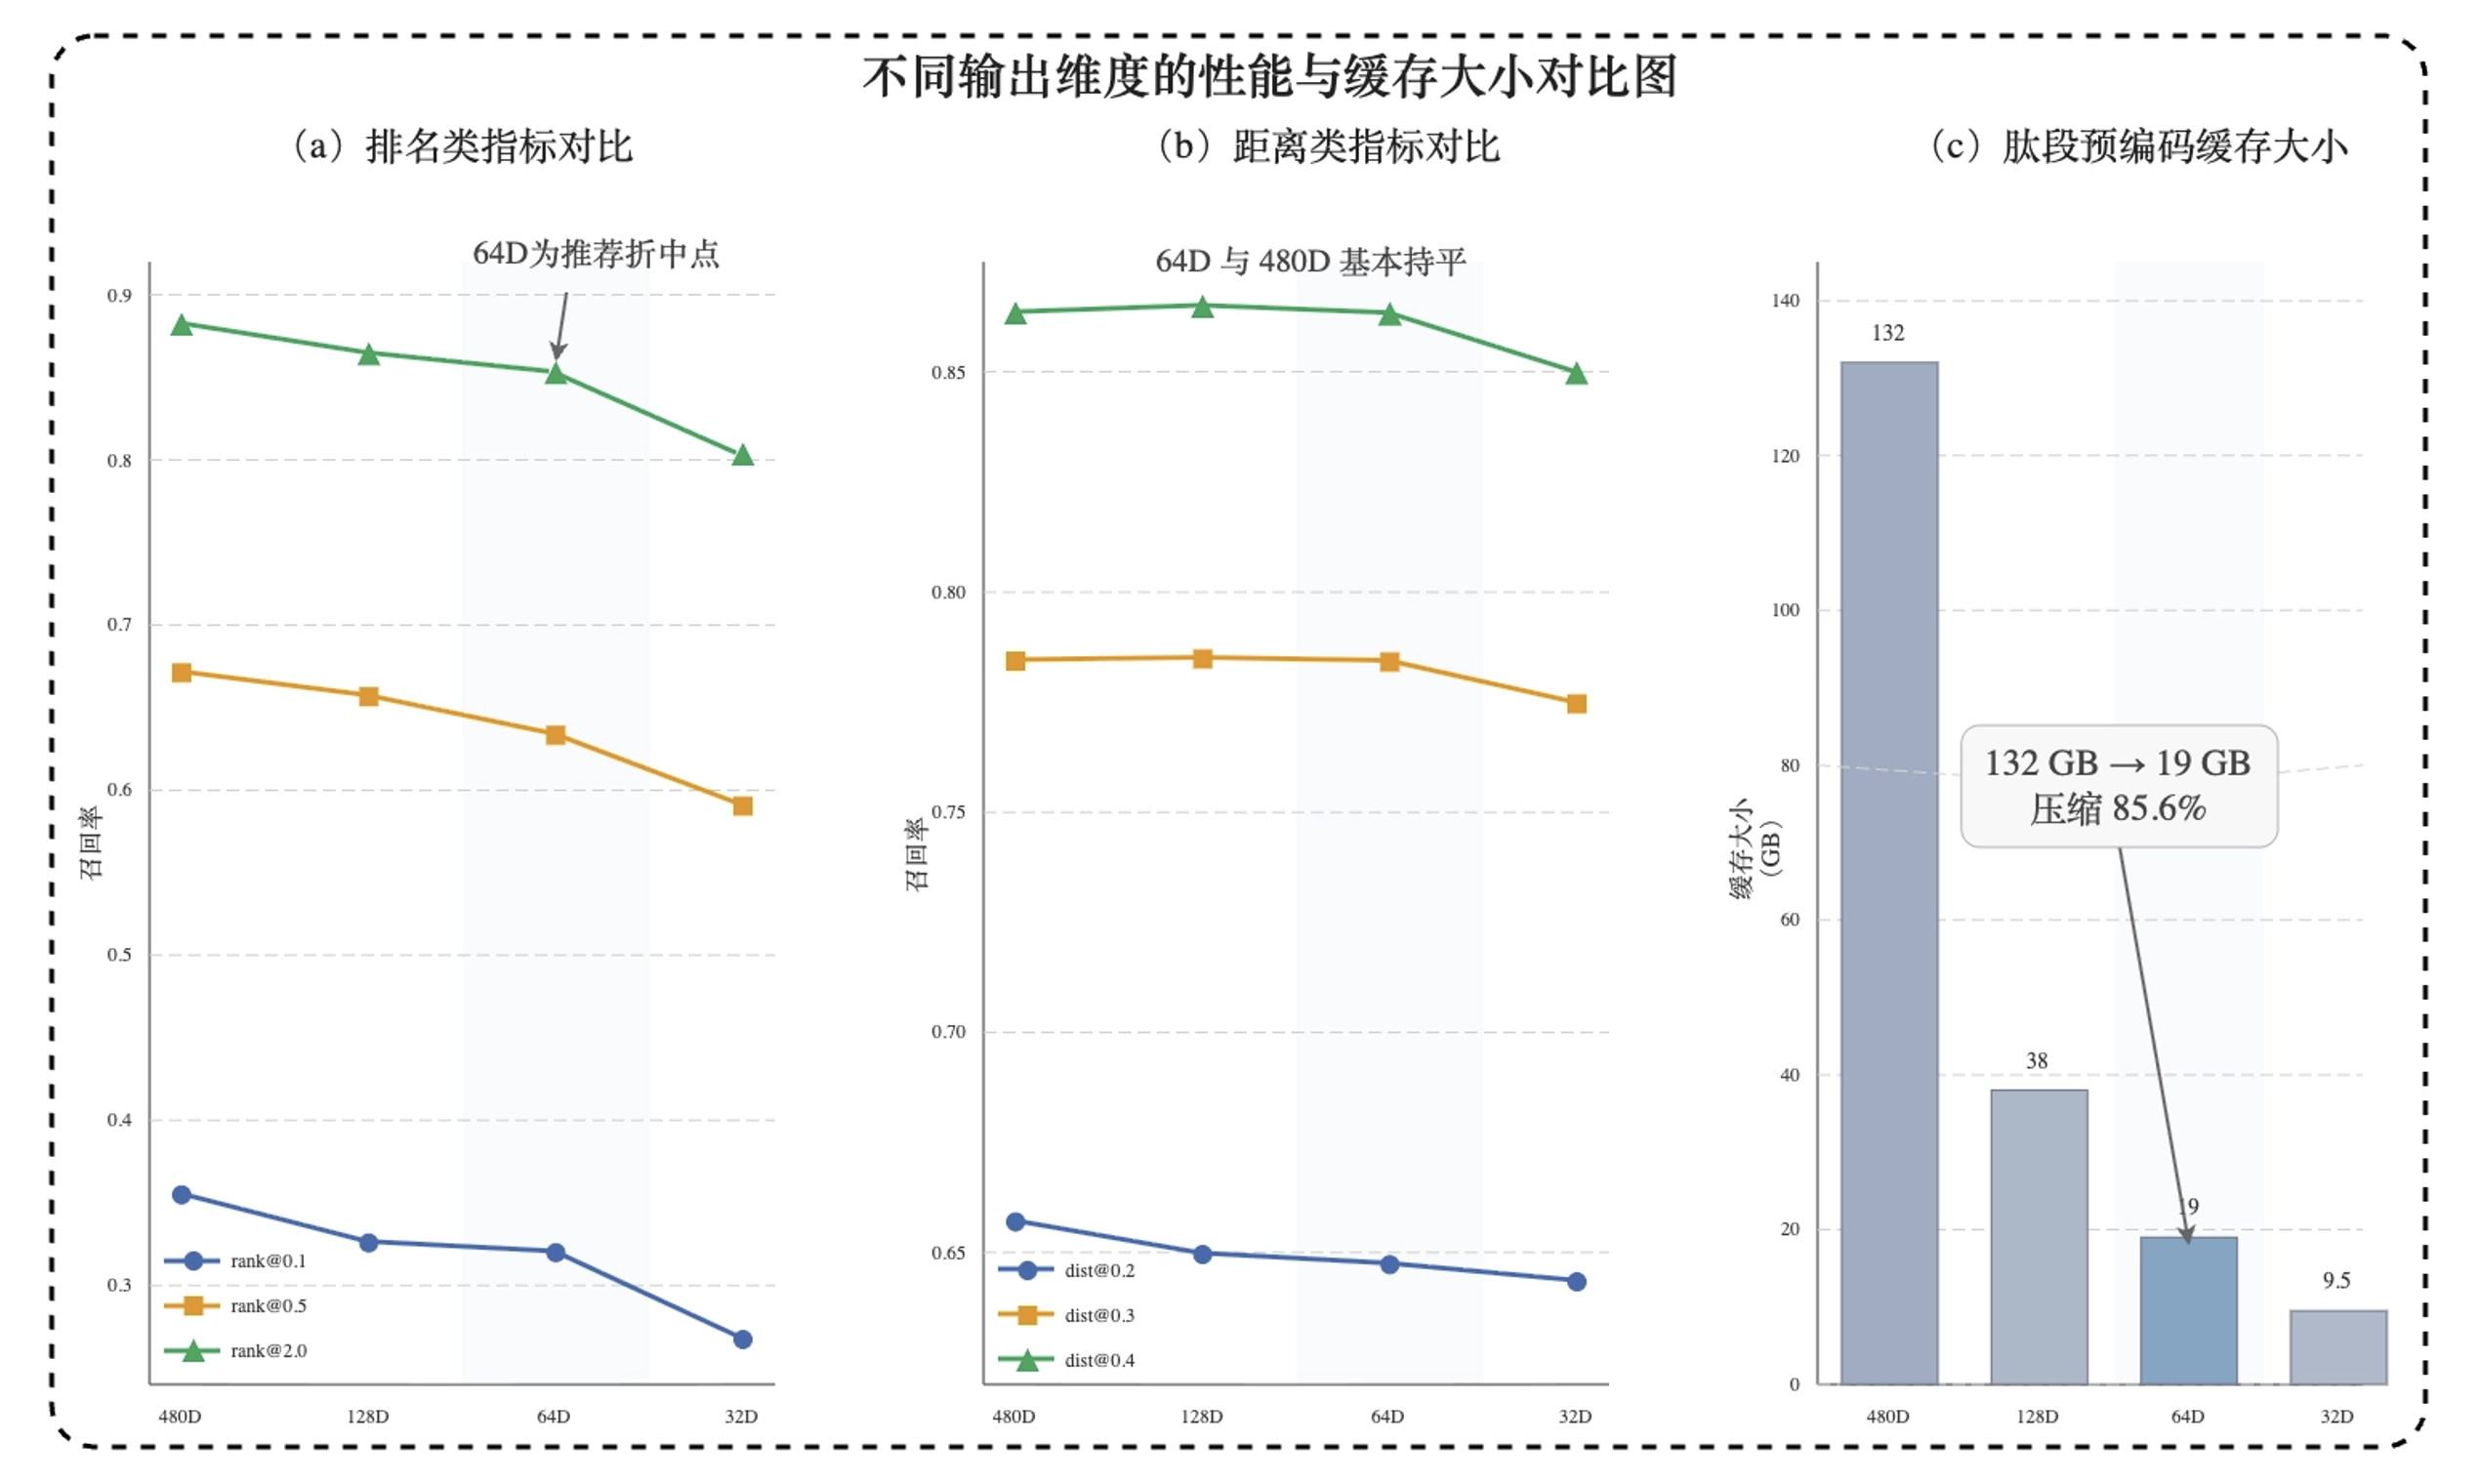
\includegraphics[width=0.90\textwidth]{figures/dimension_comparison.png}
%     \caption{不同输出维度综合比较图}
%     \label{fig:dimension-comparison}
% \end{figure}

\subsection{不同维度模型的整体性能比较}

为分析输出维度对模型性能的影响，本文比对了 480D、128D、64D 和 32D 四种配置在 rank-recall 与 distance-recall 指标上的表现，结果汇总于表~\ref{tab:dimension-performance}。

\begin{table}[htbp]
    \centering
    \caption{不同输出维度模型性能比较}
    \label{tab:dimension-performance}
    \begin{tabular}{ccccccc}
        \toprule
        输出维度 & rank@0.1 & rank@0.5 & rank@2.0 & dist@0.2 & dist@0.3 & dist@0.4 \\
        \midrule
        480D & 0.3548 & 0.6710 & 0.8820 & 0.6569 & 0.7843 & 0.8633 \\
        128D & 0.3257 & 0.6566 & 0.8641 & 0.6495 & 0.7848 & 0.8648 \\
        64D  & 0.3198 & 0.6332 & 0.8460 & 0.6472 & 0.7841 & 0.8631 \\
        32D  & 0.2672 & 0.5903 & 0.8820 & 0.6433 & 0.7746 & 0.8497 \\
        \bottomrule
    \end{tabular}
\end{table}

从 rank-recall 来看，随输出维度逐步压缩，rank@0.1 和 rank@0.5 整体呈现下降趋势，表明维度缩减会在一定程度上削弱模型对高优先级候选肽段的排序质量。其中，32D 的降幅更为明显，提示过度的压缩可能损害模型对细粒度候选差异的分辨力。

从 distance-recall 来看，128D 和 64D 与原始 480D 之间的差距很小，尤其在 dist@0.3 和 dist@0.4 两项上几乎持平。64D 模型的 dist@0.3 为 0.7841，与 480D 的 0.7843 极为接近；dist@0.4 为 0.8631，与 480D 的 0.8633 也基本一致，说明 64D 虽降低了表示维度，但仍较完整地维持了原始共享嵌入空间的邻域结构。

\begin{figure}[htbp]
    \centering
    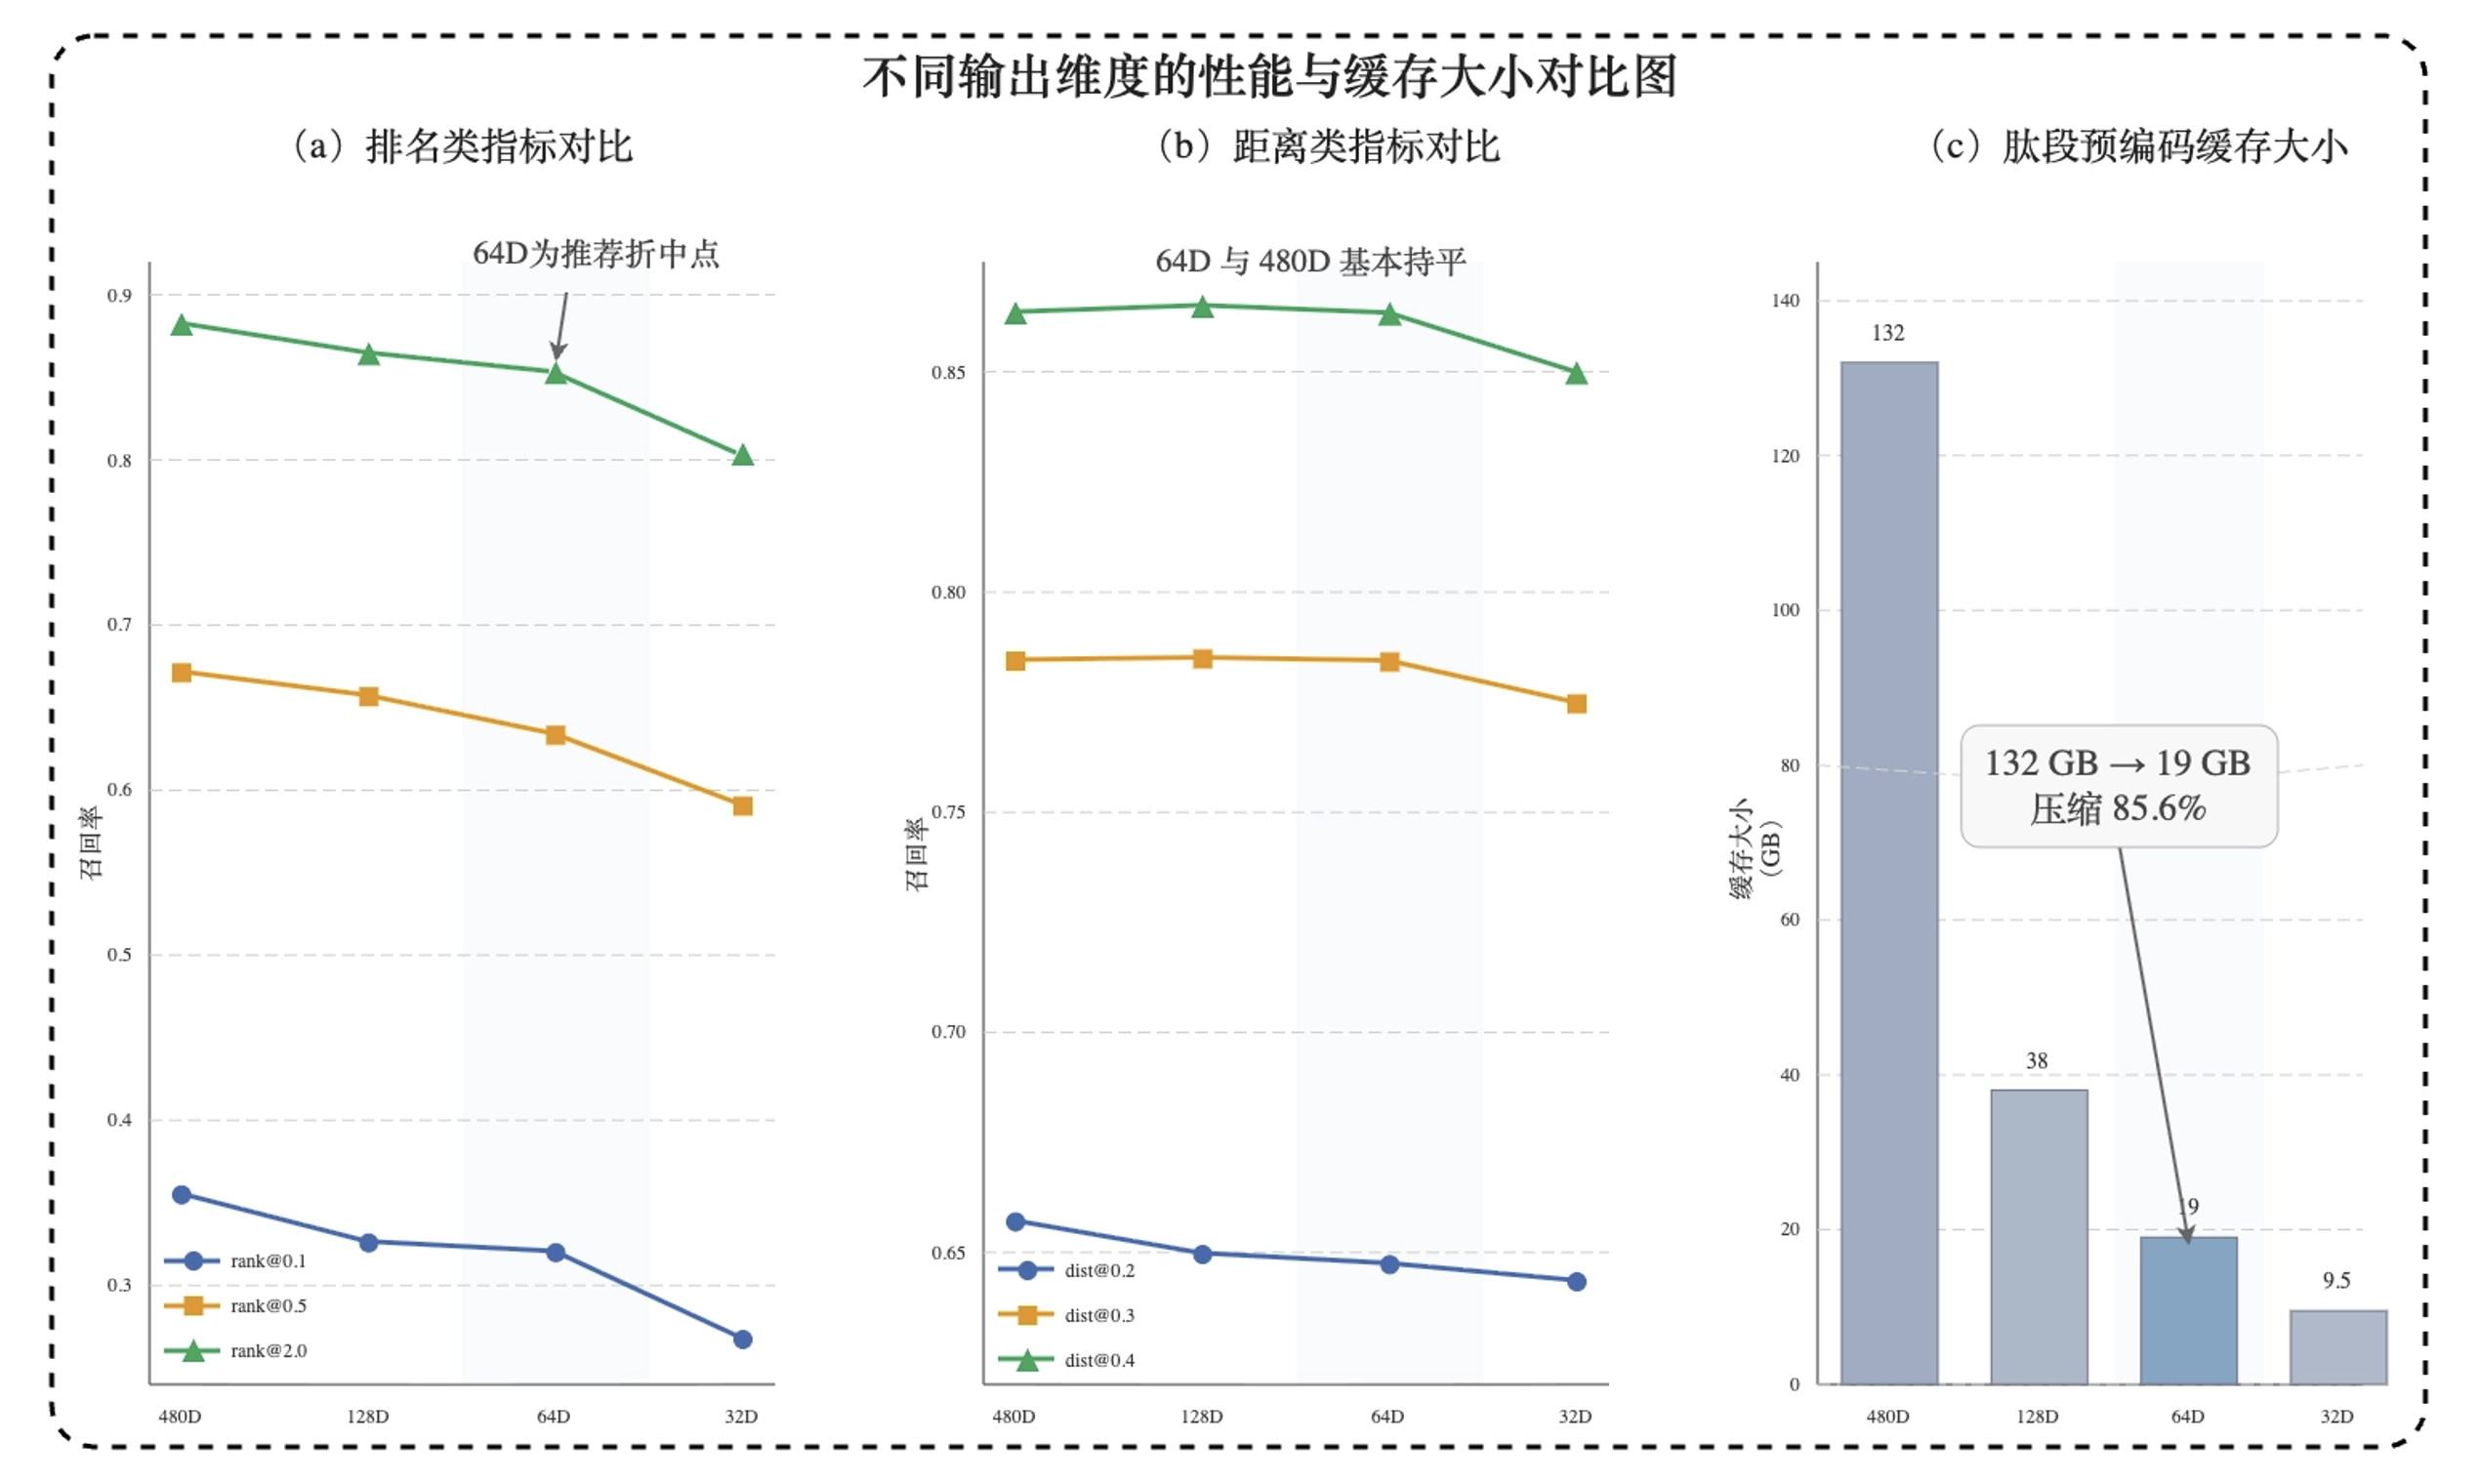
\includegraphics[width=0.90\textwidth]{figures/dimension_comparison.png}
    \caption{不同输出维度综合比较图}
    \label{fig:dimension-comparison}
\end{figure}

\subsection{不同维度模型的缓存成本比较}

除预测性能外，缓存规模是本文关切的另一项核心指标。表~\ref{tab:dimension-cache-size} 列出了不同输出维度下肽段预编码缓存的规模。

\begin{table}[htbp]
    \centering
    \caption{不同输出维度对应缓存规模比较}
    \label{tab:dimension-cache-size}
    \begin{tabular}{ccc}
        \toprule
        输出维度 & 缓存规模 & 相对 480D 的变化 \\
        \midrule
        480D & 132 GB & 基准 \\
        128D & 38 GB  & 明显降低 \\
        64D  & 19 GB  & 降低约 85.6\% \\
        32D  & 9.5 GB & 进一步降低 \\
        \bottomrule
    \end{tabular}
\end{table}

可见，输出维度与缓存规模基本呈线性关系。480D 模型约 132 GB 的缓存体积难以直接适配普通单机部署；128D 可将缓存压缩至 38 GB，但存储和加载成本仍然偏高；64D 进一步降至 19 GB，在资源占用上已明显更适合部署；32D 虽缓存最小，但需权衡前述性能上的损失。

\subsection{64 维方案的综合优势分析}

\begin{figure}[htbp]
    \centering
    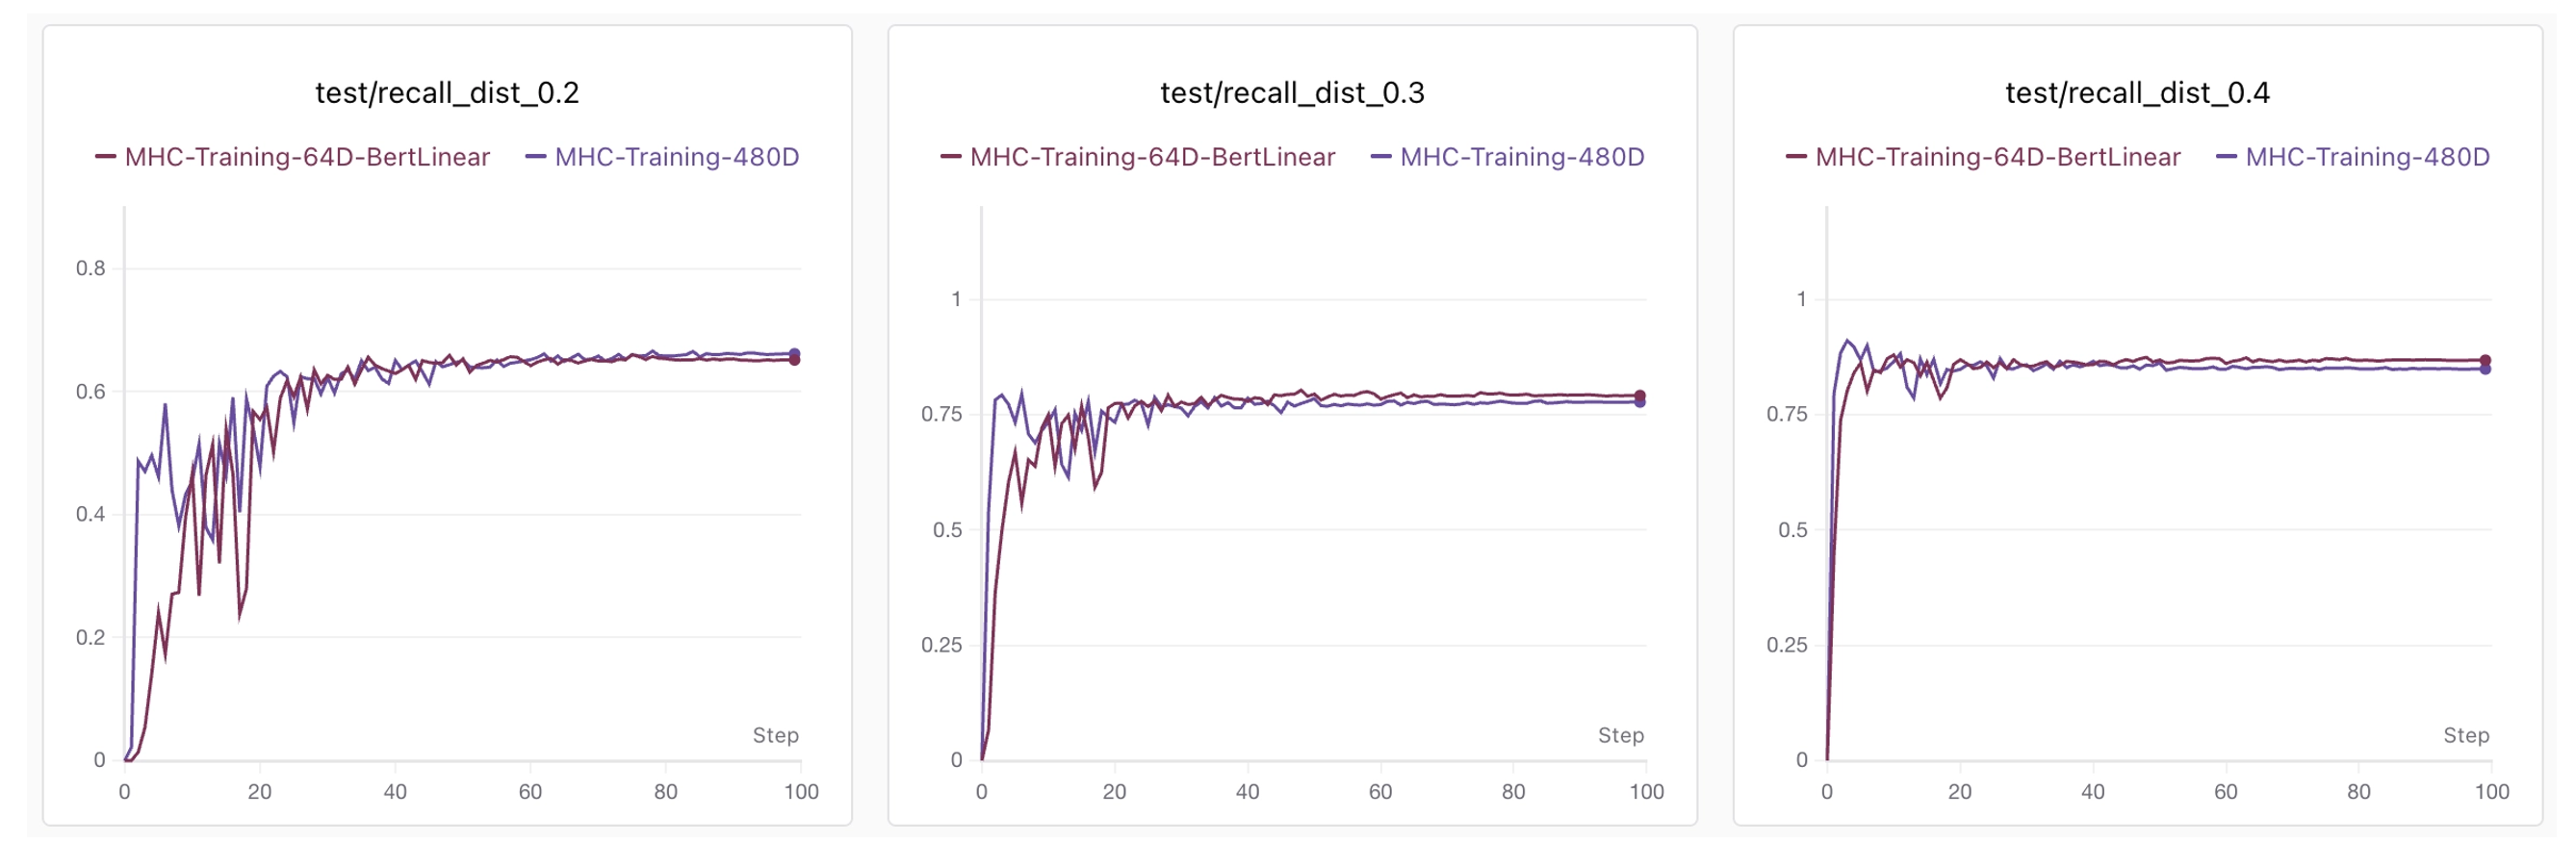
\includegraphics[width=1.0\textwidth]{figures/64d_vs_480d.png}
    \caption{64D 方案相对 480D 的压缩与 recall\_dist\_0.3 性能比较图}
    \label{fig:64d-vs-480d}
\end{figure}

综合性能与缓存成本来看，64D 是当前实验条件下较优的输出维度。一方面，它将缓存规模从 132 GB 压缩至 19 GB，显著缓解了大规模肽段库的存储压力；另一方面，其 distance-recall 指标与 480D 几无差别，说明模型的核心空间结构保持稳定。

与 128D 相比，64D 在性能损失可控的条件下额外削减了约一半缓存体积；与 32D 相比，64D 虽缓存略大，但模型表现更稳健。因此，64D 在“性能保持”与“存储压缩”之间取得了更合理的平衡。基于这一结论，后续的 Linear/MLP 对比、剪枝实验以及缓存压缩实验均以 64D 模型作为主要研究对象。

\section{线性与非线性降维模型比较分析}

\subsection{实验目的与比较对象}

在确定 64D 为主要压缩目标后，本文进一步对比 MHC-64D-BertLinear 与 MHC-64D-BertMLP 两种降维模型。两类模型的结构已在第 3.3 节中说明，此处不再赘述，而将重点放在二者在常规预测指标和下游缩库辅助搜库任务中的实验表现上。

本实验旨在判断：在相同的输出维度下，结构更轻量的 Linear 模型是否即可满足任务需求，还是具备更强非线性表达能力的 MLP 模型能带来额外增益。

\subsection{常规预测指标比较}

MHC-64D-BertLinear、MHC-64D-BertMLP 与原始 MHC-480D 在 Top-0.1\%、Top-0.5\% 和 Top-2.0\% 三个 rank-recall 指标上的整体差异不大。与此同时，在 recall\_dist\_0.2、recall\_dist\_0.3 和 recall\_dist\_0.4 等基于欧氏距离阈值的召回率上，两种 64 维模型与 480D 模型之间同样未表现出明显差距，尤其当阈值从 0.1 放宽至 0.3 后，三者的表现更为接近。

\begin{figure}[htbp]
    \centering
    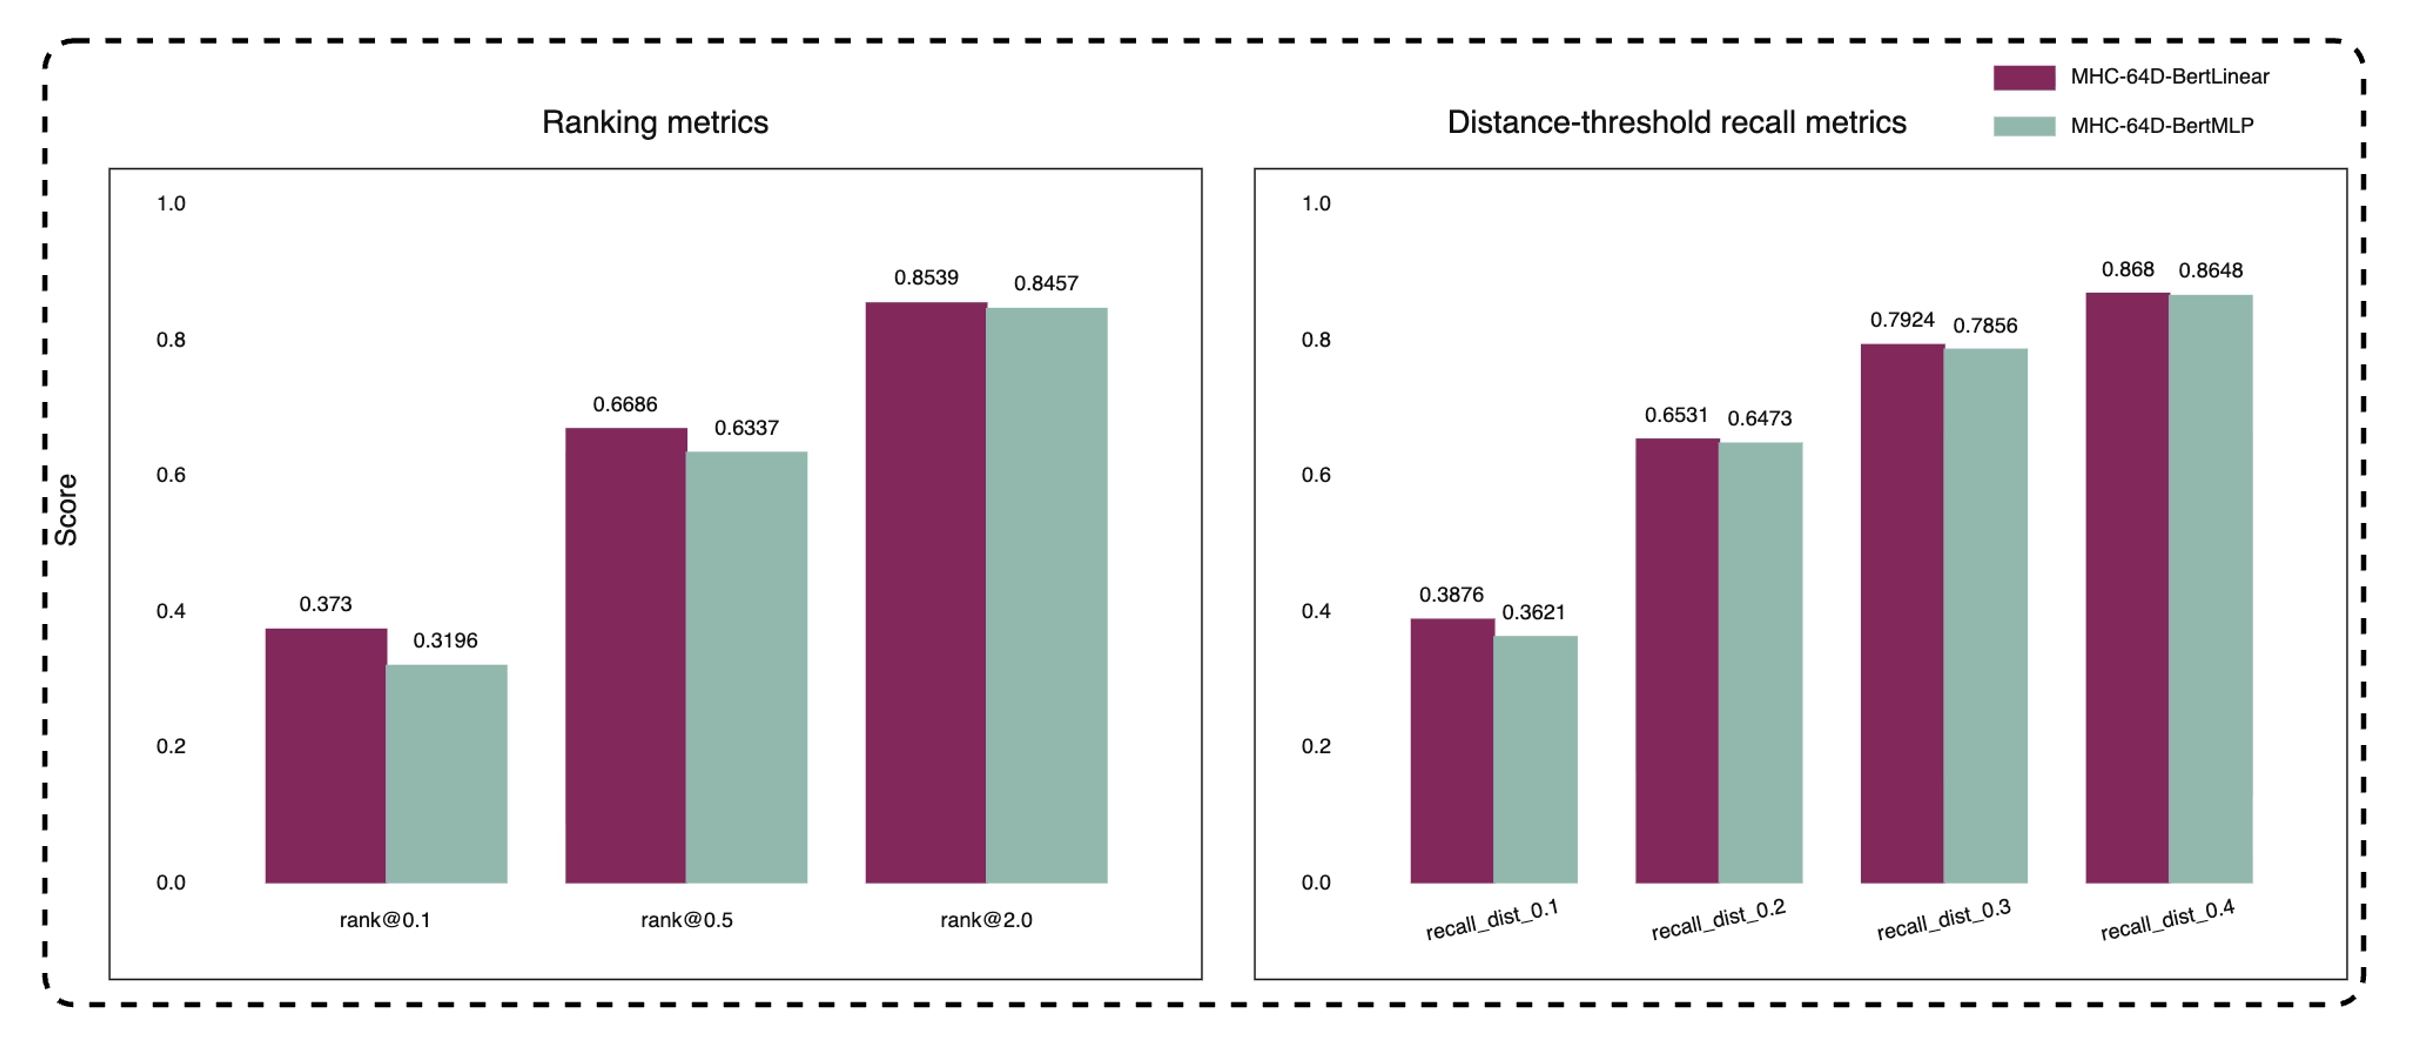
\includegraphics[width=0.85\textwidth]{figures/linear_mlp_metrics.png}
    \caption{Linear 与 MLP 常规指标对比图}
    \label{fig:linear-mlp-metrics}
\end{figure}

图~\ref{fig:linear-mlp-metrics} 显示，Linear 与 MLP 在常规预测指标上的差别微小，两者均能在 64 维条件下维持较好的候选筛选能力和嵌入空间结构。这说明，对当前 FennOmix.MHC 的特征表示而言，64 维已足以承载主要任务信息，更复杂的非线性映射并未在常规指标上体现出明显优势。

因此，仅凭 rank-recall 和 distance-recall 等常规指标，Linear 与 MLP 两类降维策略均具备可用性，二者的优劣还需结合下游缩库辅助搜库任务加以判定。

\subsection{下游缩库辅助搜库结果比较}

\begin{figure}[htbp]
    \centering
    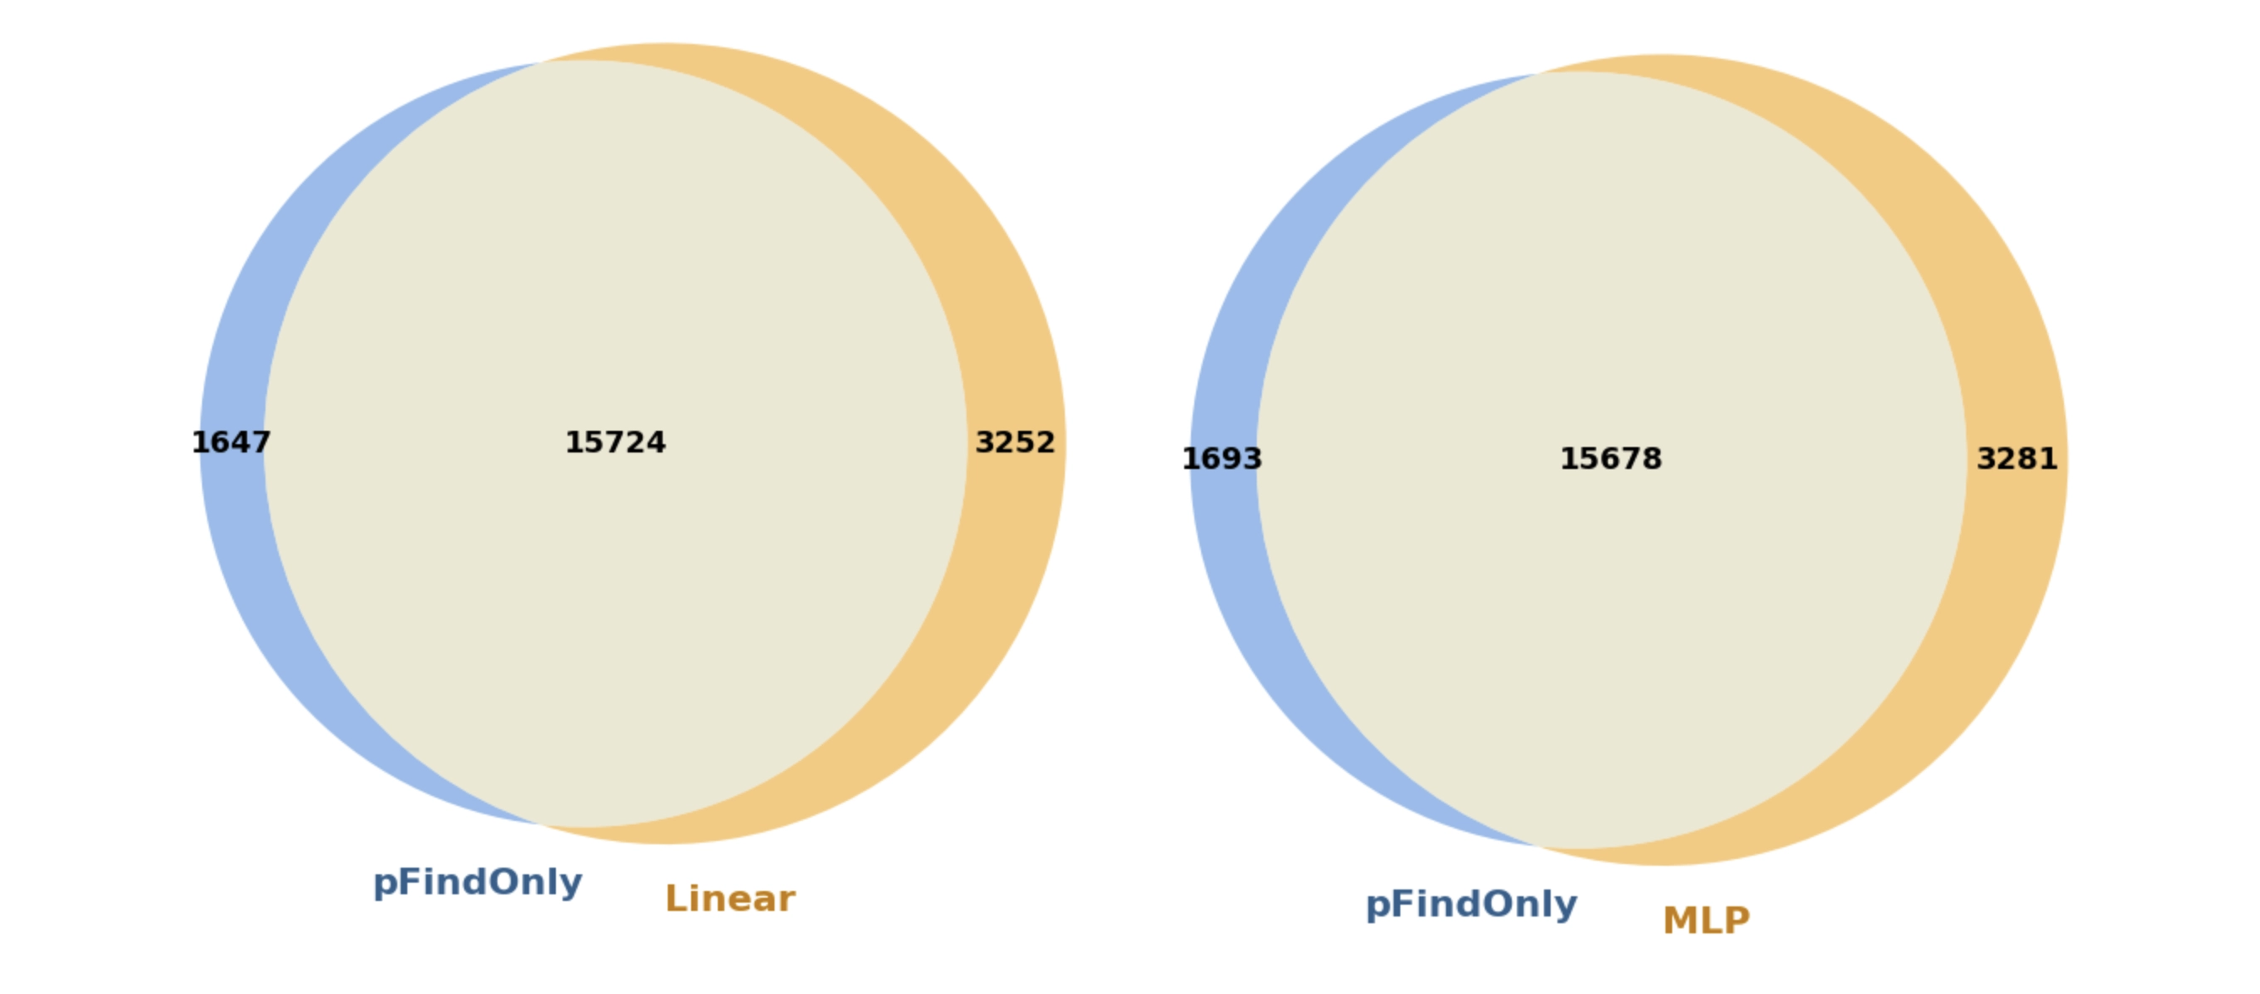
\includegraphics[width=0.85\textwidth]{figures/downstream_search_result.png}
    \caption{下游缩库辅助肽段搜库结果对比图}
    \label{fig:downstream-search-result}
\end{figure}

为更真实地评判两类模型的应用价值，本文进一步引入基于等位基因的缩库辅助数据库检索任务进行对比。具体做法是：对同一批 MS/MS 数据，在已知 HLA 等位基因的条件下分别执行 Direct Search 和 Model-assisted Search 两种流程，后者先由 FennOmix.MHC 对候选肽段进行打分与筛选，构建等位基因特异的缩减数据库，再通过 pFind 实施检索。随后，在肽段层面对两条流程的输出进行 overlap 分析，结果如图~\ref{fig:downstream-search-result} 所示。

\begin{figure}[htbp]
    \centering
    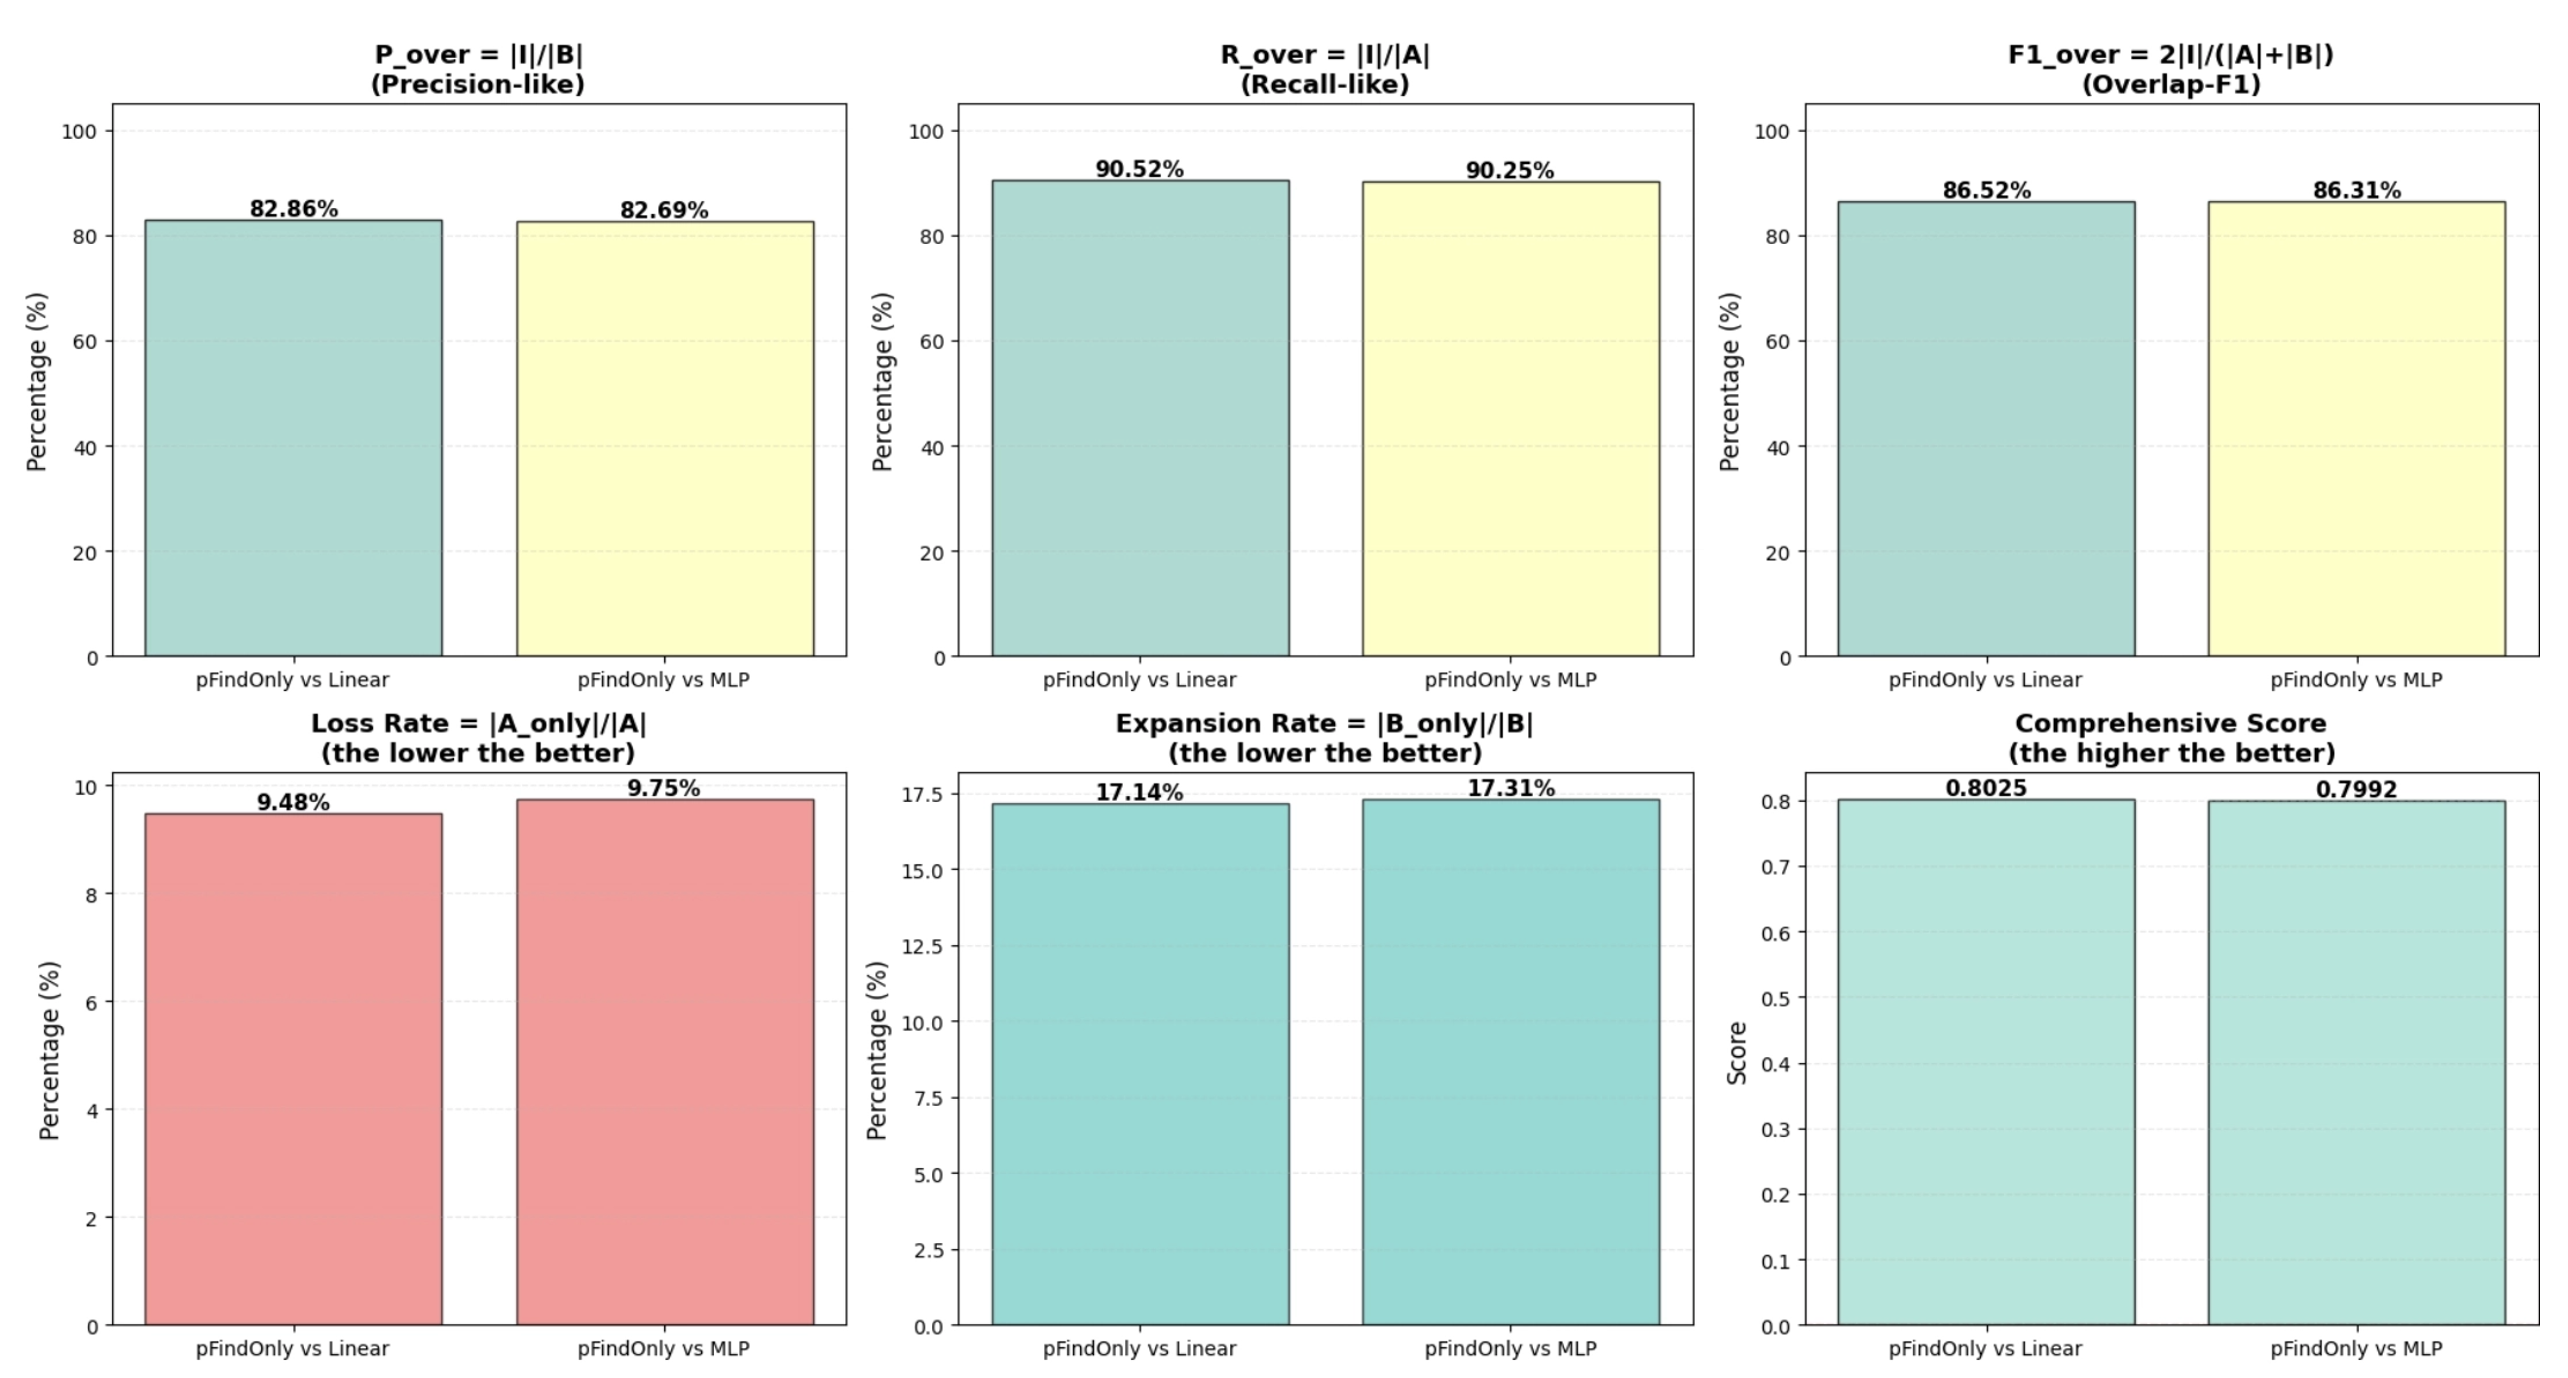
\includegraphics[width=1.0\textwidth]{figures/overlap_scores.png}
    \caption{Linear vs MLP Overlap Scores 指标对比图}
    \label{fig:overlap-scores}
\end{figure}

从图~\ref{fig:overlap-scores} 所示的 Overlap Scores 评价结果来看，Linear 与 MLP 在下游任务中的整体表现相近，但 Linear 在 Precision-like、Recall-like、Overlap-F1、Loss Rate、Expansion Rate 和 Comprehensive Score 六项指标上均呈现出一致的轻微优势。这表明，尽管 MLP 具有更强的非线性表达能力，但在当前任务与数据条件下，这一能力并未转化为更优的下游检索效果。

该结果也印证，当常规预测指标接近时，下游任务评价具有重要参考价值。对于本文所关注的部署场景，模型不仅需要在测试集上维持较好的召回率，还应在真实缩库流程中尽量保留基线检索结果并减少额外差异。Linear 在该任务中的稳健表现，使其更适合被选作默认降维方案。

\subsection{结果分析与结论}

综合常规指标与下游任务结果，Linear 与 MLP 均能在 64D 条件下保持较好的模型性能，但 Linear 在工程部署和应用效果上更具优势：结构更简单、参数量更少、部署成本更低；在常规指标接近的前提下，Linear 在下游 overlap 六项指标中整体略优；且 Linear 的实现与维护更为直接，更适宜作为系统默认模型。

因此，本文最终选定 MHC-64D-BertLinear 作为后续剪枝、缓存压缩与系统部署分析的主要模型基础。

\section{剪枝实验结果分析}

\subsection{剪枝重要性分析结果}

在 64D 线性模型的基础上，本文进一步分析 Transformer 结构中各组件的贡献差异，以判断模型是否存在可剪枝的冗余。实验结果如图~\ref{fig:attention-head-importance} 所示，不同层及不同注意力头的重要性分布并不均衡，表明模型结构中确实存在一定的冗余空间。

\begin{figure}[htbp]
    \centering
    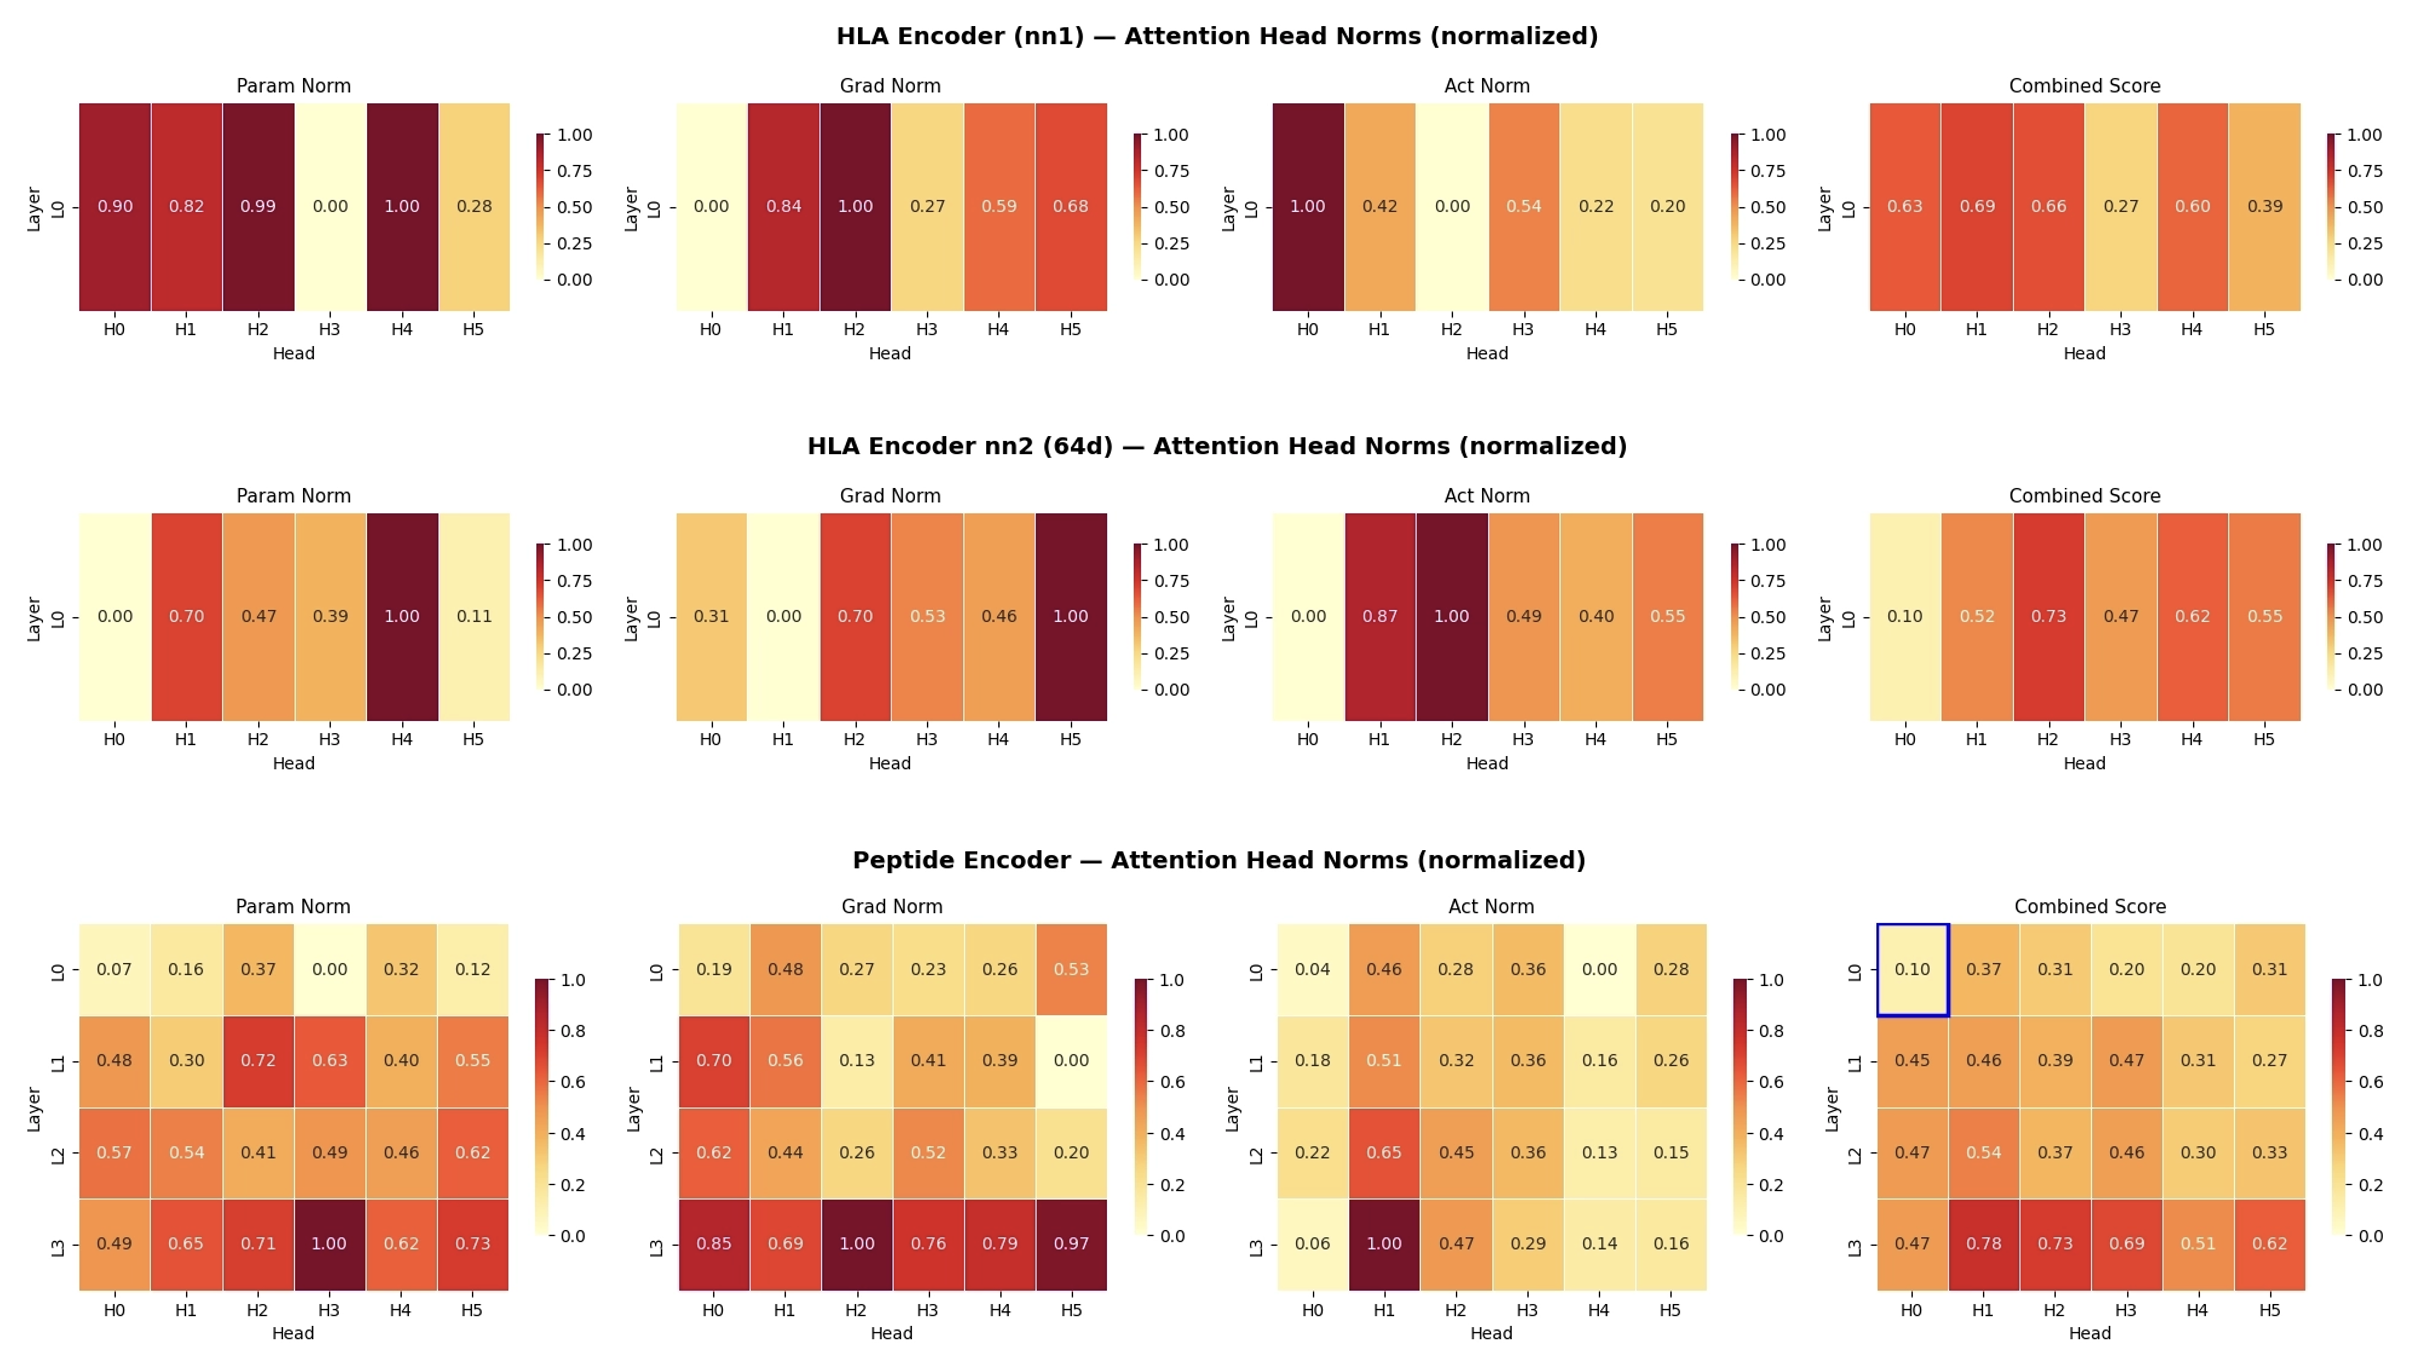
\includegraphics[width=1.0\textwidth]{figures/attention_head_importance.png}
    \caption{注意力头重要性热图}
    \label{fig:attention-head-importance}
\end{figure}

在 HLA Encoder 中，nn1 的 H0、H2、H3、H5 以及 nn2 的 H2、H4、H5、H3 贡献突出，应优先保留。在 Peptide Encoder 中，L0--H0 的 Combined Score 在全模型中最低，各类范数也普遍偏低，几乎未提供有效表征，因而被视为强剪枝候选；L0--H3 同样贡献偏弱，也可作为优先剪枝对象。与之相对，L3 中的 H1、H2、H3、H5 以及同层的 H0、H4 重要性较高，剪枝时应予以保留。

这些结果表明，FennOmix.MHC 的不同注意力头并非等价贡献，部分结构承担了主要表征功能，而另一些则贡献较弱，这为基于重要性分析的剪枝提供了实验依据。

\subsection{剪枝前后性能比较}

完成重要性分析后，本文对低贡献结构实施了剪枝，并测试了剪枝后模型的预测性能。由图~\ref{fig:pruning-performance} 可见，剪枝前后模型的整体性能差异较小，主要评价指标未出现显著下滑。

这一结果说明，当前模型结构中确有一部分可压缩的冗余。通过合理选择低重要性注意力头或前馈层进行剪枝，可以在基本保持模型预测能力的同时降低结构复杂度。对于后续部署而言，剪枝可作为降维之外的补充优化手段，进一步削减推理阶段的冗余计算。

\begin{figure}[htbp]
    \centering
    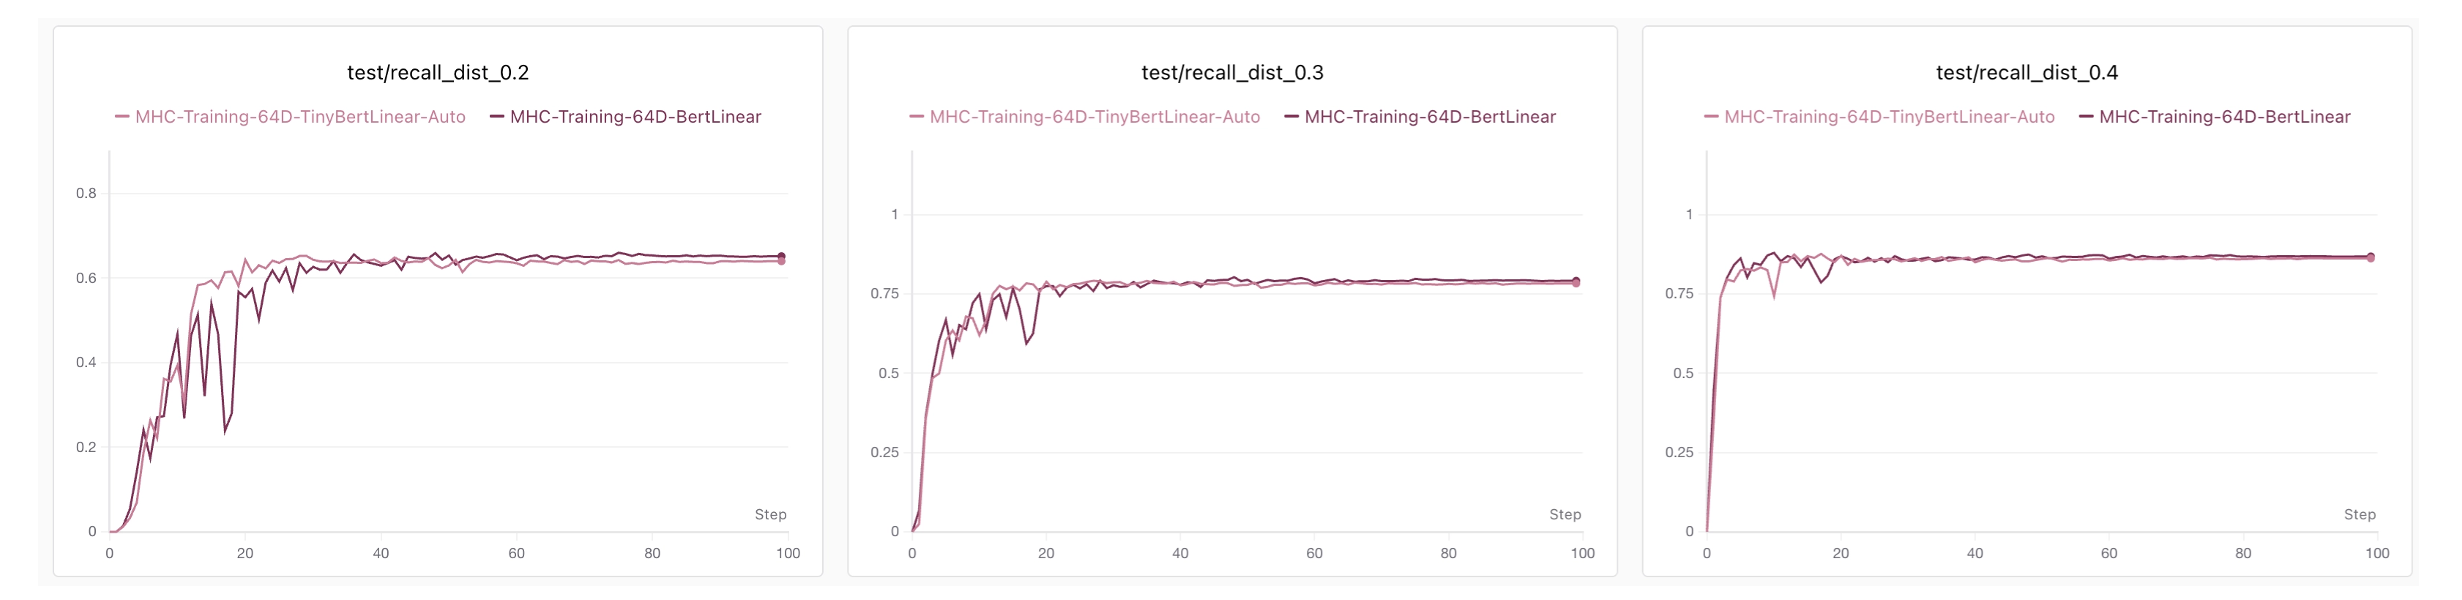
\includegraphics[width=1.0\textwidth]{figures/pruning_performance.png}
    \caption{模型剪枝前后性能对比图}
    \label{fig:pruning-performance}
\end{figure}

\subsection{剪枝结果讨论}

剪枝实验的主要价值并不在于显著提升预测性能，而在于证实模型结构仍有进一步压缩的空间。与输出维度压缩重点降低缓存成本不同，剪枝直接对模型结构做减法，有助于减少推理时的计算量。不过，目前的剪枝实验仍以验证可行性为主，对不同剪枝比例、组合策略以及剪枝后实际推理加速效果的分析还不够深入。因此，我们将剪枝结果定位为一种结构冗余的验证与部署优化的初步探索，为后续更细粒度的模型压缩研究提供基础。

\section{缓存压缩与索引机制实验分析}

\subsection{64 维缓存的压缩需求}

前面的实验已经表明，64D 模型可将肽段缓存从 132 GB 压缩至 19 GB，但在 7300 万条肽段的大规模场景下，19 GB 依然会带来一定的存储、加载和传输压力。因此，在 64D float32 缓存的基础上，我们进一步检验 INT8 量化压缩与索引加载策略的实际效果。本节重点从误差、存储收益和加载方式三个角度分析其部署表现。

\subsection{INT8 量化压缩结果}

从图~\ref{fig:quantization-result} 可以看出，采用 INT8 量化后，64D 肽段向量的主体数据由 float32 的 4 Byte/维压缩为 int8 的 1 Byte/维。忽略少量缩放因子与文件头开销后，embedding 主体数据的体积可近似缩减至原来的四分之一。

误差方面，量化后的实际 MSE 约为 $7.5 \times 10^{-7}$，低于理论最大值 $2.1 \times 10^{-6}$。这说明量化压缩虽然降低了存储位宽，但对向量数值分布的扰动非常轻微。后续匹配主要依赖 HLA 与肽段嵌入间的距离关系，如此低的量化误差意味着该方法具备较好的部署可行性。

\begin{figure}[htbp]
    \centering
    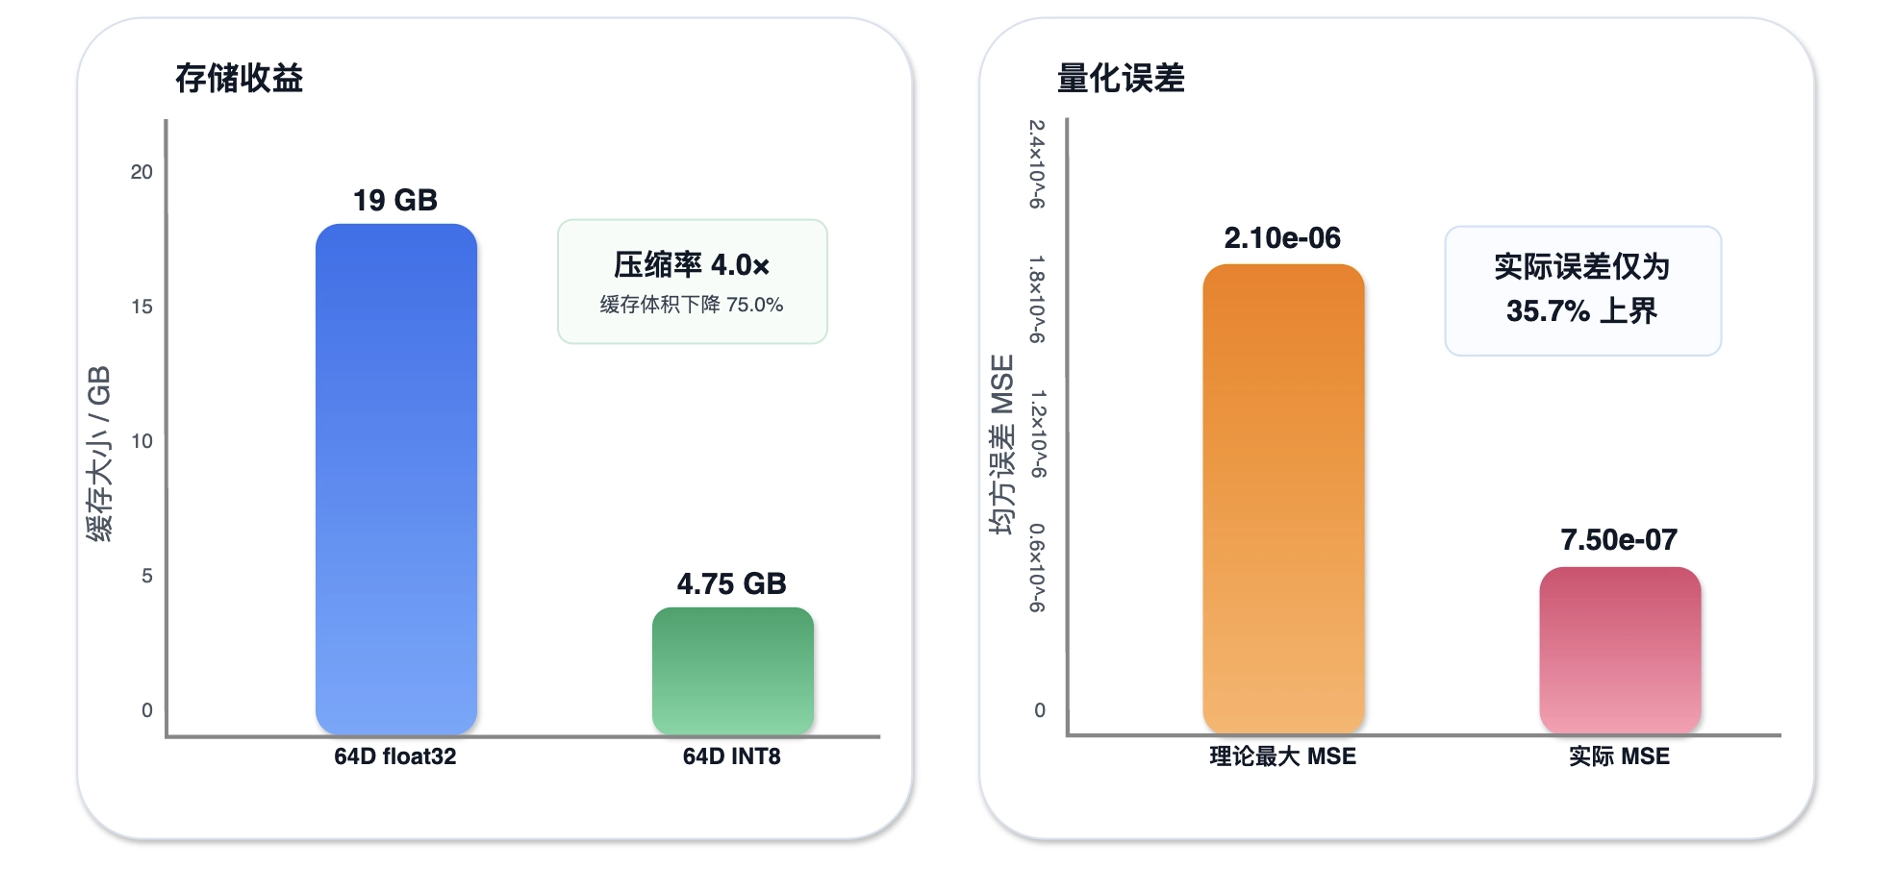
\includegraphics[width=0.80\textwidth]{figures/quantization_result.png}
    \caption{量化误差与存储收益图}
    \label{fig:quantization-result}
\end{figure}

综合来看，INT8 量化能在保持较高数值精度的同时进一步缩减缓存占用，是 64D 降维之后的一个重要补充优化。

\subsection{索引机制与加载策略分析}

\begin{figure}[htbp]
    \centering
    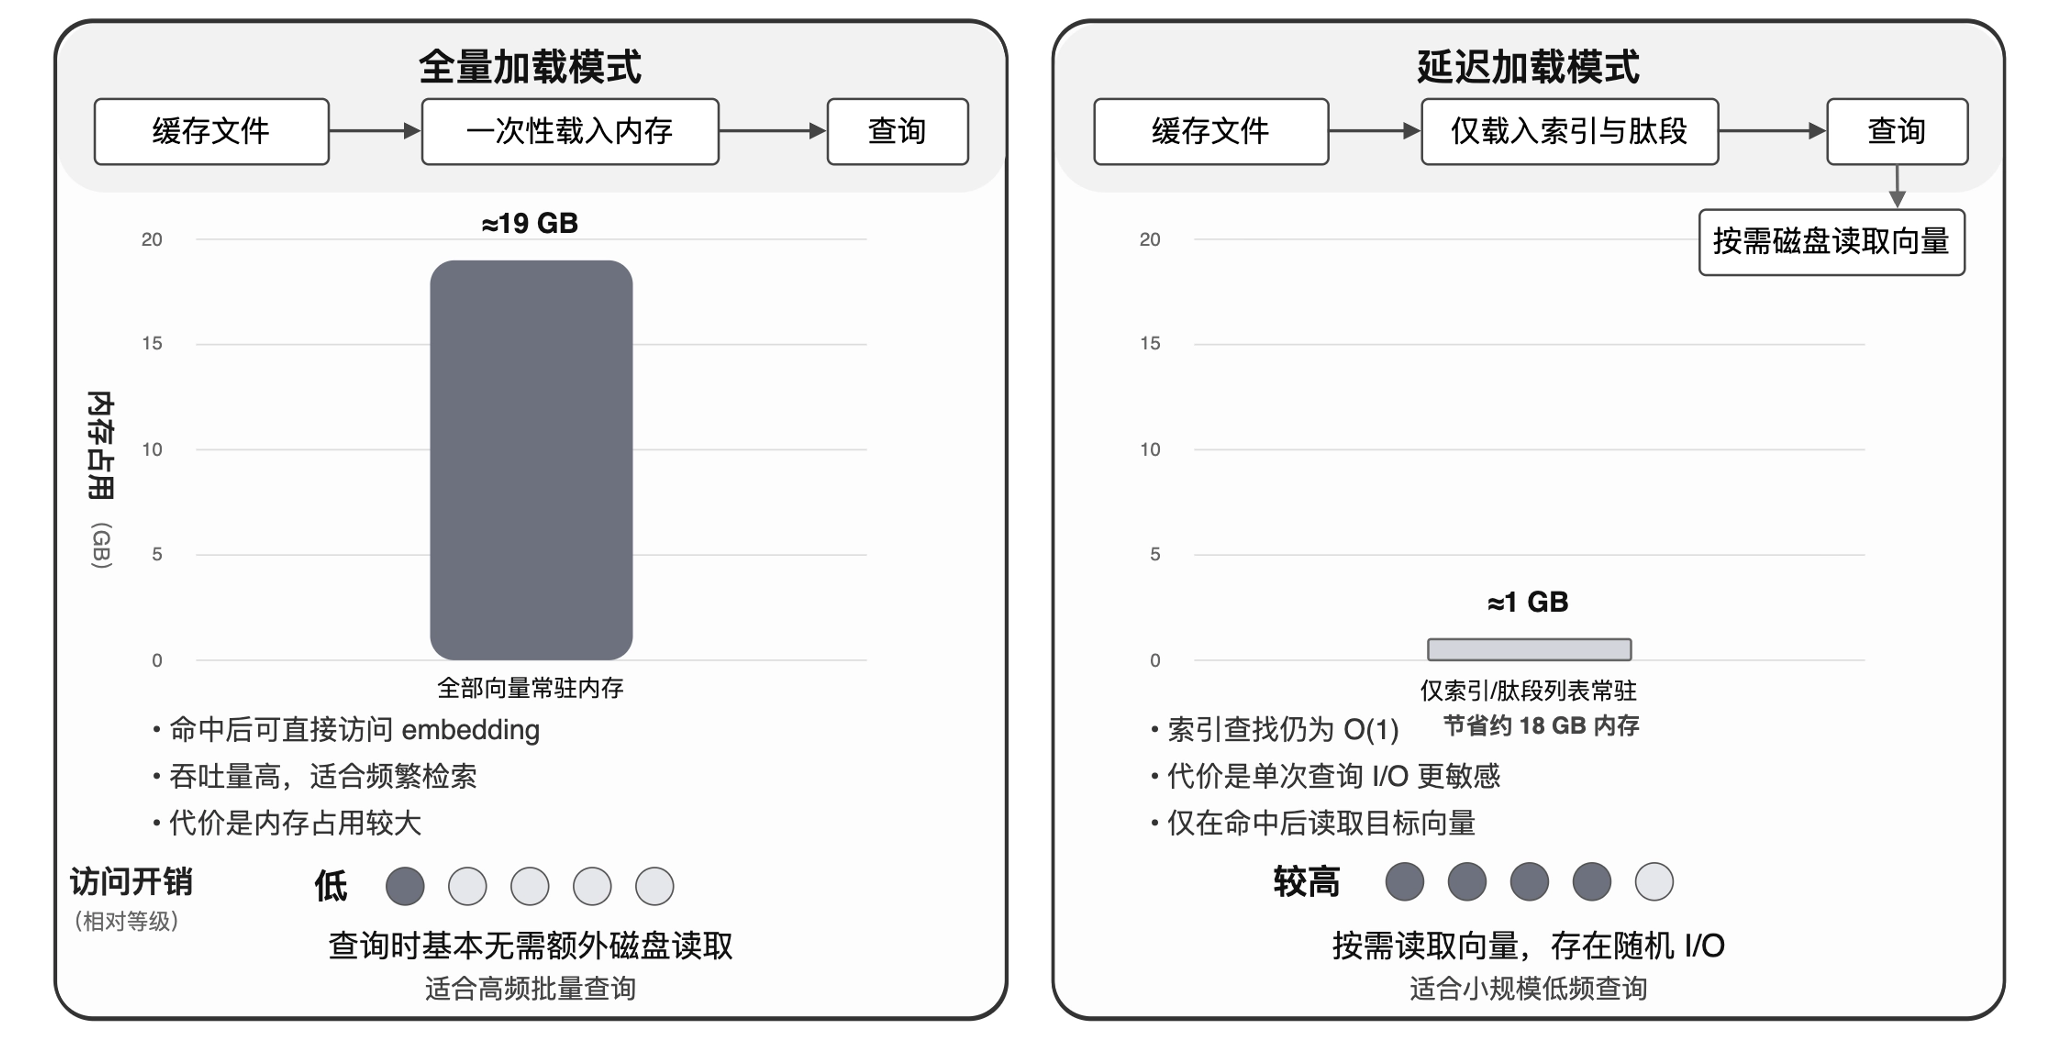
\includegraphics[width=0.80\textwidth]{figures/loading_strategy_result.png}
    \caption{全量加载与延迟加载的内存/访问开销分析图}
    \label{fig:loading-strategy-result}
\end{figure}

在索引机制层面，我们利用 peptide\_index 建立了肽段字符串到向量位置的映射，使系统在缓存命中时能够快速定位对应的嵌入向量。实验分析表明，这一设计可以避免在数千万级候选肽段中逐条搜索，让查询过程更适合大规模部署场景。

在加载策略层面，全量加载与延迟加载分别适配不同的资源条件。全量加载适合高频查询，能减少查询过程中的磁盘访问延迟；延迟加载则适合小规模查询或内存紧张的环境，仅加载肽段列表与索引，在需要时才读取对应向量。实验估算显示，延迟加载模式可节省约 18 GB 内存，能有效降低系统的常驻资源占用。

可以看出，索引与加载策略的价值不仅体现在查询速度上，也体现在部署灵活性上。系统可以根据任务规模、查询频率和硬件条件在全量加载与延迟加载之间灵活切换。

\subsection{查询链路效果分析}

在完整的查询链路中，系统优先通过索引判断输入肽段是否命中缓存：命中的肽段直接读取缓存向量，未命中的则回退到实时编码路径。随后，系统计算肽段 embedding 与目标 HLA embedding 之间的欧氏距离，并基于距离阈值或排序结果输出潜在结合肽段。

实验分析表明，这条链路能够兼顾高效性与开放性。常见的候选肽段可以受益于离线缓存和索引机制，减少重复编码开销；缓存外的新肽段则通过实时编码路径保证系统依然具备处理能力。从这个角度来看，缓存压缩与索引机制并不是孤立的优化，而是与在线预测流程共同构成了完整的部署链路。

\section{综合讨论}

\subsection{从模型精度到系统部署的统一优化路径}

本章实验结果揭示，本文所提的优化路线并非单层面的性能微调，而是从模型表示、模型结构和系统缓存三个层面逐步压低部署成本。

首先，在模型表示层面，64D 在保持 distance-recall 基本不变的前提下，将缓存规模从 132 GB 压缩至 19 GB，是当前性能与成本之间较理想的折中。其次，在降维模型选择上，Linear 与 MLP 的常规指标接近，而 Linear 在下游缩库辅助搜库任务中略占上风，故更适合作为默认方案。再次，在模型结构层面，剪枝实验揭示了模型内存在可压缩冗余，合理剪枝后性能依旧稳定。最后，在系统缓存层面，INT8 量化与索引加载机制进一步减轻了存储和内存压力，使模型更契合大规模候选肽段场景。

\subsection{实验结果的主要结论}

本章实验可归结出以下结论。第一，64D 是当前实验条件下较优的输出维度，其在 dist@0.3 和 dist@0.4 上几乎与 480D 持平，同时大幅压缩了缓存成本。第二，Linear 与 MLP 在常规预测指标上差异甚微，Linear 在下游缩库辅助搜库任务中整体略优且结构更轻量，因而更适宜作为默认降维模型。第三，剪枝实验表明 FennOmix.MHC 存在一定的结构冗余，基于重要性分析进行剪枝可在性能基本稳定的前提下降低模型复杂度。第四，INT8 量化能够进一步压缩 64D 缓存，实际 MSE 维持在较低水平；配合哈希索引和两阶段加载策略后，系统在存储、内存和访问方式上展现出更好的部署适应性。

\subsection{当前实验的局限性}

尽管本章实验验证了整体技术路线的可行性，但仍存在若干不足。首先，模型剪枝实验目前主要关注剪枝前后的性能稳定性，对不同剪枝比例、不同层级组合以及实际推理加速效果的分析尚待细化。其次，INT8 量化实验主要从误差角度论证了压缩效果，对于不同量化参数如何影响最终检索性能还可进一步探究。最后，索引与加载策略虽已完成原型验证，但在多进程、多机环境下的吞吐量、延迟和容错能力仍需更系统的测试。

因此，本文当前的实验更侧重于证明“降维—剪枝—缓存压缩—索引检索”这条路径的可行性，后续仍有必要围绕参数组合、速度收益和工程鲁棒性进行补充研究。

\section{本章小结}

本章围绕 FennOmix.MHC 的模型优化与系统部署需求，开展了系统的实验分析。首先，比较了 480D、128D、64D 和 32D 四种输出维度，结果显示 64D 在保持嵌入空间结构稳定的同时显著降低了缓存成本。其次，对比了 Linear 与 MLP 两类 64D 降维模型，发现二者常规指标接近，Linear 在下游缩库辅助搜库任务中略优，故被确定为默认降维方案。随后，剪枝实验证实模型结构中存在一定冗余，基于重要性分析的剪枝可在性能基本稳定的前提下减少模型复杂度。最后，INT8 量化、哈希索引与两阶段加载策略进一步提升了系统在大规模肽段库场景下的可部署性。

整体而言，本章的实验结果印证了本文所提优化路线的可行性与应用价值，也为第四章进一步展开系统设计与部署分析提供了实验依据。